%\documentclass{beamer}
\documentclass[a4paper,9pt]{beamer}
\usepackage{colortbl}
%\documentclass{12pt}
\usepackage[english]{babel}
\usepackage{beamerthemesplit} % new
\usepackage{amsmath}
\usepackage{amssymb}
\usepackage{latexsym}
%\usetheme[showpagenr=tue]
%\newcounter{saveenumi}
%\newcounter{saveenumii}
%\newcounter{saveenumiii}
%\insertframnumber
%\inserttotalframenumber
%\usepackage[latin1]{inputenc}
% or whatever
\mode<presentation>
{
 \usetheme{Frankfurt}
 \usecolortheme{rose}
  \setbeamercovered{transparent}
}


\usepackage{times}
\usepackage[T1]{fontenc}
%\usepackage{fontenc}
%\usepackage{fourier}

%%%%%%%%%%%%%%%%%%%%%%%%%%%%%%%%%%%%%%%%%%%%%%%%%%

\title{eTourPlan: A Knowledge-Based\\ Tourist Route and Activity Planner}
\subtitle{Thesis Oral Defence for MCS Degree Program}
\author{Tshering Dema}
\institute{\normalsize{Supervisors: Dr. Harold Boley,\\
\hspace{1.4in} Dr. Przemyslaw Rafal Pochec}}

\begin{document}
\begin{frame}
  \titlepage
\end{frame}
%%%%%%%%%%%%%%%%%%%%%%%%%%%%%%%%%%%%%%%%%%%%%%%%%%

%\frame{\frametitle{Acknowledgement}
%\begin{itemize}
 %\item  Canadian International Development Agency (CIDA)
 %\item  Bhutan Project
 %\item  University of New Brunswick
%\end{itemize} 
%}


\frame{\frametitle{Outline}
\begin{enumerate}
%\begin{columns}[c] % the "c" option specifies center vertical alignment
%\column{.5\textwidth} % column designated by a command
\item Introduction \vspace*{0.3cm} 
%\item Problems \vspace*{0.3cm} 
%\item Objectives \vspace*{0.3cm} 
\item Background \vspace*{0.3cm} 
%\item Testbed Architecture \vspace*{0.3cm} 
%\column{.5\textwidth}
%\item Testbed Architecture \vspace*{0.3cm} 
\item Rule Languages and Tools \vspace*{0.3cm} 
\item Knowledge Base Design: Ontology and Facts \vspace*{0.3cm} 
\item Knowledge Base Design: Rules \vspace*{0.3cm} 
\item Evaluation of eTourPlan on the Bhutan KB \vspace*{0.3cm} 
\item Conclusion and Future Work \vspace*{0.3cm} 
%\item References \vspace*{0.3cm} 
%\end{columns}

\end{enumerate}
}
%%%%%%%%%%%%%%%%%%%%%%%%%%%%%%%%%%%%%%%%%%%%%%%%%%
%slide 2
\section{1. Introduction}

\subsection{1.1 Motivation}
\frame{\frametitle{1.1 Motivation}
\begin{itemize}
\item \vspace{0.3cm} 
\item Tourism is the world's largest and fastest growing industry
\vspace{0.3cm}
\item The World Tourism Organization predicts that one billion international tourists will travel by the year 2010
\vspace{0.3cm}
\item A highly competitive business for tourism destinations all over the world
\vspace{0.3cm}
\item There are many conventional tourism service providers which are competively trying to provide the best travel plans and recommendations to thier customers%\pause
\item \vspace{0.3cm} 

%\pause
%\item \vspace{0.2cm} 
%GOAL: Provide QoS test-bed and investing characteristics of real-time Internet traffic 
%on the heterogeneous networks.
%\item \vspace{0.2cm} 
%How much bandwidth do we need to provide good quality for a given video?
\end{itemize}
}
%%%%%%%%%%%%%%%%%%%%%%%%%%%%%%%%%%%%%%%%%%%%%%%%%
\subsection{1.2 Motivation}
\frame{\frametitle{1.2 Goals}
\begin{itemize}
%\item \vspace{0.2cm} 
%There is growing popularity of Real-time Internet traffic such as video and audio streams.\\
%However, when congestion occurs, all traffic suffers the same impairments, \\
% e.g, increasing delay, more variable delay , and packet drops
%\pause
%\item \vspace{0.2cm} 
%Quality of Service (QoS) mechanisms (Differentiated Service) are necessary.
%\pause
\item \vspace{0.3cm} 
To provide QoS test-bed and investigating characteristics of real-time Internet traffic 
on the heterogeneous networks.
\item \vspace{0.3cm}
To investigate measurement techniques to measure performance.
\item \vspace{0.3cm}
To configure what bandwidth and burst size is required to stream MPEG2 video through the DiffServ domain.
\end{itemize}
}
%%%%%%%%%%%%%%%%%%%%%%%%%%%%%%%%%%%%%%%%%%%%%%%%%%

%\subsection{1.2 Hotspot}
%\frame{\frametitle{1.2 Hotspot}
%\begin{itemize}
%\item \vspace{0.2cm}
%Broadband Internet connection
%\item \vspace{0.2cm}
%Public Hotspot for everyone

%\end{itemize}
%}
%%%%%%%%%%%%%%%%%%%%%%%%%%%%%%%%%%%%%%%%%%%%%%%%%%
%\section{2. Problems}
%\subsection{2.1 The Problem}
%\frame{\frametitle{2.1 The Problems}
%\begin{itemize}
%\pause \item \vspace{0.2cm} real-time streaming applications require minimum bandwidth and guaranteed QoS.  Real-time Internet traffic, such as video and audio, is always bandwidth hungry and delay sensitive
%\item \vspace{0.2cm} The Internet traditionally was designed for best-effort data delivery
%\pause 
%\item \vspace{0.2cm} Increasing delay, More variable delay, and Packet loss
%\pause 
%\item \vspace{0.2cm} Real-time Internet traffic, such as video and audio, is always bandwidth hungry and delay sensitive
%\end{itemize}

%}
%///////////////////////////////////////////////////////
%\section{3. Objectives}
%\subsection{3.1 Research Objectives}
%\frame{\frametitle{3.1 Objectives}

%\begin{itemize}
%\item \vspace{0.2cm} 
%Packet scheduler (Hierarchical Token Bucket) is to classify packets and to manage the bandwidth
%\pause
%\item \vspace{0.2cm} 
%Packet marker is to categorize packets
%\pause
%\item \vspace{0.2cm}
%Policer to regulate packets
%\pause
%\item \vspace{0.2cm} 
%Evaluating QoS techniques for transmission of real-time video that use a Diffserv mechanism
%\end{itemize}
%}
%#========================================
%Background Discussion : Concepts and Terminologies

\section{2. Background}
\subsection{2.1 Methodology for QoS Mechanism}
\frame{\frametitle{2.1 Methodology for QoS Mechanism}
 \begin{itemize}
  \item \vspace{0.2cm} Bandwidth Broker (BB):\\
            to manage heterogeneous network.
  \item \vspace{0.2cm} TungaBaskaraRao's Thesis:\\
    End-to-End QoS Signaling for Real-Time Data Streams.
  %\item \vspace{0.2cm} Edge Router (ER):\\
   % Policing, marking, and classifying IP traffic.
  %\item \vspace{0.2cm} Core Router (CR):\\
   % Forwarding IP traffic
\item \vspace{0.2cm} Policer regulates packets
\begin{itemize}
                     \item \vspace{0.2cm} rate parameter
                     \item \vspace{0.2cm} burst parameter  
              \end{itemize}
\item \vspace{0.2cm} Packet Marker categorizes packets
\item \vspace{0.2cm} Packet scheduler manages the bandwidth
              \begin{itemize}
                     \item \vspace{0.2cm} Expedited Forwarding (EF) traffic
                     \item \vspace{0.2cm} Best Effort (BE) traffic  
              \end{itemize}
 \end{itemize}
}
%%%%%%%%%%%%%%%%%%%%%%%%%%%%%%%%%%%%%%%%%%%%%%%%%%%
\frame{\frametitle{2.2 DiffServ Testbed Architecture}
%ER is to accept and filter the incoming packets: policing and marking IP traffic.
\begin{columns}[c]
\column{.7\textwidth}
\begin{figure}[h] 
\includegraphics[width=7cm, height=6.8cm]{QoStestbed.jpg}
\end{figure}
 \column{.3\textwidth} 
\begin{figure}[h] 
\includegraphics[width=3.8cm, height=2.7cm]{r1.jpg}
%\caption{IP packets in the Linux Kernel on the ER}
\end{figure}
%CR is to carry on packet scheduling and forwarding

\begin{figure}[h] 
\includegraphics[width=3.8cm, height=2.7cm]{r2.jpg}
%\caption{IP packets in the Linux Kernel on the ER}
\end{figure}
\end{columns}
}
%//////////////////////////////////////////////////

%//////////////////////////////////////////////////
%\subsection{4.2 Token Bucket Mechansim}
%\frame{\frametitle{4.2 Token Bucket Mechansim}
% \begin{itemize}
%  \item \vspace{0.2cm} Token
%  \item \vspace{0.2cm} Bucket
% %\pause \item \vspace{0.2cm} Burst
% \end{itemize}
%}
%//////////////////////////////////////////////////
%\section{5. Testbed Architecture}
%\subsection{5.1 TungaBaskaraRao's Thesis}
%\frame{\frametitle{5.1 TungaBaskaraRao's Thesis}
% \begin{itemize}
% \item \vspace{0.2cm} End-to-End QoS Signaling for Real Time Data Streams
% \item \vspace{0.2cm} Originally, a QoS domain was designed by TungaBaskaraRao
% \item \vspace{0.2cm} Implementing Bandwidth Broker (QoS Agent)
% \item \vspace{0.2cm} Implementing QoS Client
% \end{itemize}
%}
%//////////////////////////////////////////////////
%\subsection{5.2 Testbed Architecture}
%\frame{\frametitle{5.2.1 Testbed Architecture}
%\begin{figure}[h] 
%\includegraphics[width=10cm, height=7.7cm]{QoStestbed.jpg}
%\end{figure}
%}
%||||||||||||||||||||||||||||||||||||||||||||||||||||


%//////////////////////////////////////////////////////////////
\section{3. Experiments}
\subsection{3.1 Testing the QoS domain}
\frame{\frametitle{3.1.1 Testing the DiffServ domain}
\begin{columns}[c]
 \column{.7\textwidth}
\begin{figure}[h] 
\includegraphics[width=7cm, height=7cm]{QoStestbed.jpg}
\end{figure}
\column{.3\textwidth}
 \begin{itemize}
 \item \vspace{0.2cm} Measurement tool : Iperf
 \item \vspace{0.2cm} Video Sender transmits {\color {red} 3Mbits} data to Video Receiver
 \item \vspace{0.2cm} Background Srouce transmits {\color {red} 5Mbits} to Video Reciever
 \item \vspace{0.2cm} Wireless link's {\color {red} Total Throughput} is {\color {red} 5.5 Mbits}
 \end{itemize}
\end{columns}
}
%%%%%%%%%%%%%%%%%%%%%%%%%%%%%%%%%%%%%%
\frame{\frametitle{3.1.2 Background Source 192.168.10.10 client report}
\begin{figure} [p]%tbph
\centering
\begin{tabular}{|l|}
\hline
[cnsr\.@localhost \.~\.]\$ /usr/bin/iperf -c {\color {blue} 131.202.243.5} -p 55555 -u -b {\color {blue} 5M} -t 30\\
-----------------------------------------------------------\\
Client connecting to 131.202.243.5, UDP port 55555\\
Sending 1470 byte datagrams\\
UDP buffer size:   108 KByte (default)\\
-----------------------------------------------------------\\
\.[  3\.] local 192.168.10.10 port 32772 connected with 131.202.243.5 port 55555\\
\.[  3\.]  0.0-30.0 sec  17.9 MBytes  5.00 Mbits/sec\\
\.[  3\.] Sent 12757 datagrams\\
\.[  3\.] WARNING: did not receive ack of last datagram after 10 tries.\\
\.[cnsr\.@localhost \.~ \.]\$\\
\hline
\end{tabular}
%\caption{Background Source 192.168.10.10 client report}
\end{figure} 
}
%%%%%%%%%%%%%%%%%
\frame{\frametitle{3.1.3 QoS client 192.168.11.10 client report}
\begin{figure} [p]
\centering
\begin{tabular}{|l|}
\hline
\.[cnsr\.@localhost videos\.]\$ /usr/bin/iperf -c {\color {blue} 131.202.243.5} -p 55556 -u -b {\color {blue} 3M} -t 30\\
------------------------------------------------------------\\
Client connecting to 131.202.243.5, UDP port 55556\\
Sending 1470 byte datagrams\\
UDP buffer size:   108 KByte (default)\\
------------------------------------------------------------\\
\.[  3\.] local 192.168.11.10 port 32772 connected with 131.202.243.5 port 55556\\
\.[  3\.]  0.0-30.0 sec  10.7 MBytes  3.00 Mbits/sec\\
\.[  3\.] Sent 7655 datagrams\\
\.[  3\.] Server Report:\\
\.[  3\.]  0.0-30.0 sec  10.6 MBytes  2.96 Mbits/sec  0.109 ms 104/ 7654 (1.4\%)\\
\.[  3\.]  0.0-30.0 sec  1 datagrams received out-of-order\\
\.[cnsr\.@localhost videos\.]\$\\
\hline
\end{tabular}
%\caption{QoS client 192.168.11.10 client report}
\end{figure}
}
%%%%%%%%%%%%%%%%%%%%%%%%%%%%%%%%%%%%%%%%%%%%%%%%%
\frame{\frametitle{3.1.4 Server report for {\color {red} background traffic}}
\begin{figure} [tbph]
\centering
\begin{tabular}{|l|}
\hline
\.[cnsr\.@ib\.214m05 \.~\.]\$ /usr/bin/iperf -s -p 55555 -u -i 5\\
------------------------------------------------------------\\
Server listening on UDP port 55555\\
Receiving 1470 byte datagrams\\
UDP buffer size:   108 KByte (default)\\
------------------------------------------------------------\\
\.[  3\.] local 131.202.243.5 port 55555 connected with 131.202.240.63 port 32772\\
\.[  3\.]  0.0- 5.0 sec  1.87 MBytes  3.14 Mbits/sec  0.706 ms  679/ 2012 (34\%)\\
\.[  3\.]  5.0-10.0 sec  3.08 MBytes  5.17 Mbits/sec  1.362 ms   44/ 2199 (2\%)\\
\.[  3\.]  5.0-10.0 sec  44 datagrams received out-of-order\\
\.[  3\.] 10.0-15.0 sec  2.93 MBytes  4.92 Mbits/sec  6.334 ms    0/ 2093 (0\%)\\
\.[  3\.] {\color {red} 15.0-20.0 sec}  1.39 MBytes  {\color {red} 2.34 Mbits/sec}  3.420 ms  938/ 1932 (49\%)\\
\.[  3\.] 15.0-20.0 sec  81 datagrams received out-of-order\\
\.[  3\.] {\color {red} 20.0-25.0 sec}  1.38 MBytes  {\color {red} 2.32 Mbits/sec}  4.098 ms 1128/ 2115 (53\%)\\
\.[  3\.] {\color {red} 25.0-30.0 sec}  1.40 MBytes  {\color {red} 2.36 Mbits/sec}  4.541 ms 1131/ 2133 (53\%)\\
\.[  3\.]  0.0-30.6 sec  12.2 MBytes  3.35 Mbits/sec  2.948 ms 4020/12756 (32\%)\\
\.[  3\.]  0.0-30.6 sec  126 datagrams received out-of-order\\
read failed: Connection refused\\
\hline
\end{tabular}
\end{figure}
}
%%%%%%%%%%%%%%%%%%%%%%%%%%%%%%%%%%%%%%%%%%%%%%%%%%
\frame{\frametitle{3.1.5 Server report for {\color {red} EF traffic}}
\begin{figure} [tbph]
\centering
\begin{tabular}{|l|}
\hline
\.[cnsr\.@ib\.214m05 \.~\.]\$ /usr/bin/iperf -s -p 55556 -u -i 5\\
------------------------------------------------------------\\
Server listening on UDP port 55556\\
Receiving 1470 byte datagrams\\
UDP buffer size:   108 KByte (default)\\
------------------------------------------------------------\\
\.[  3\.] local 131.202.243.5 port 55556 connected with 131.202.240.63 port 32772\\
\.[  3\.]  {\color {red} 0.0- 5.0 sec}  1.64 MBytes  {\color {red} 2.75 Mbits/sec}  2.036 ms  105/ 1276 (8.2\%)\\
\.[  3\.]  {\color {red} 5.0-10.0 sec}  1.77 MBytes  {\color {red} 2.98 Mbits/sec}  1.925 ms    0/ 1266 (0\%)\\
\.[  3\.] {\color {red} 10.0-15.0 sec}  1.80 MBytes  {\color {red} 3.02 Mbits/sec}  1.671 ms    0/ 1286 (0\%)\\
\.[  3\.] {\color {red} 15.0-20.0 sec}  1.79 MBytes  {\color {red} 3.00 Mbits/sec}  0.200 ms    0/ 1275 (0\%)\\
\.[  3\.] {\color {red} 20.0-25.0 sec}  1.79 MBytes  {\color {red} 3.00 Mbits/sec}  0.129 ms    0/ 1276 (0\%)\\
\.[  3\.] {\color {red} 25.0-30.0 sec}  1.79 MBytes  {\color {red} 3.00 Mbits/sec}  0.105 ms    0/ 1275 (0\%)\\
\.[  3\.]  0.0-30.0 sec  10.6 MBytes  2.96 Mbits/sec  0.109 ms  104/ 7654 (1.4\%)\\
\.[  3\.]  0.0-30.0 sec  1 datagrams received out-of-order\\
read failed: Connection refused\\
\hline
\end{tabular}
\end{figure}
}
%%%%%%%%%%%%%%%%%%%%%%%%%%%%%%%%%%%%%%%%%%%%%%%%%%%%%%%%
\subsection{3.2 Characteristic of Packet Scheduler (HTB qdisc)}
\frame{\frametitle{3.2.1 Configuring Packet Scheduler (HTB qdisc)}
\begin{columns}[c]
 \column{.5\textwidth}
\begin{figure}[h] 
\includegraphics[width=5.5cm, height=5.7cm]{QoStestbed.jpg}
\end{figure}
\column{.5\textwidth}
\begin{figure} [tbph]
\centering
\begin{tabular}{|l|}
\hline
 Clip2.mpeg \\
 MPEG2 compression video, \\
 320$\times$240, 29.970 fps, \\
 MPEG layer-2, duration 92s.\\
 File size = 8043364 bytes.\\
\hline
\end{tabular}
\caption{clip2.mpg specification}
\end{figure}

\begin{figure} [tbph]
\centering
\begin{tabular}{|l|}
\hline
Estimated average rate (bps):\\
file size/duration.\\
%(8043364$\times$8)b/92s = 699422bps\\
%699422bps / 1000 = 699kbits/sec\\
Estimated average rate for \\
clip2.mpeg is 699kbits/sec\\
\hline
\end{tabular}
%\caption{Estimated average rate for clip2.mpg}
\end{figure}
\begin{itemize} 
\item VLC at the Video Sender, 
\item VLC at the CR,
\end{itemize}
\end{columns}
}
%%%%%%%%%%%%%%%%%%%%%%%%%%%%%%%%%%%%%%%%%%%%%%%%%%%%%%%%%%%%%%%%%%%%%
\frame{\frametitle{3.2.2 HTB to manage the bandwidth}
%ER is to accept and filter the incoming packets: policing and marking IP traffic.
\begin{columns}[c]
 \column{.43\textwidth} 
\begin{figure}[t]
\centering
\includegraphics[width=5cm, height =3.5cm]{nnqdisc.jpg}
\caption{The qdisc-class hierarchy of the configuration used for the research}
\end{figure}
\column{.57\textwidth}
\begin{table} [b]
\caption{Link Specification at the Edge Router}
\centering
\begin{tabular}{|l|l|l|l|}
\hline
  Link & BW(Mbps) & EF  & BE \\
\hline
  192.168.10.0/24 &  94.5 &44.5& 50\\
\hline
  192.168.11.0/24 & 9.5 &4.5&5\\
\hline
  192.168.12.0/24 & 94.5& 44.5&50 \\
\hline
\end{tabular} 
%\caption{Link Specification at the Edge Router}
\end{table}

\begin{table} [b]
\caption{Link Specification at the Core Router}
\centering
\begin{tabular}{|l|l|l|l|}
\hline
%\rowcolor{red}%%%%%%%%%%%%%%%%%%%%%%%%%%%%%%%%66666666666666666666666666666666666666666666666666666
  Link &  BW(Mbps)& EF & BE \\
\hline
   192.168.12.0/24 & 94.5 & 44.5 & 50 \\
\hline
  131.202.240.0/22 & 5.5&3.5&2 \\
\hline
\end{tabular} 
%\caption{Link Specification at the Core Router}
\end{table}
\end{columns}
}
%%%%%%%%%%%%%%%%%%%%%%%%%%%%%%%%%%%%%%%%%%%%%%%%%%%%%%%%%%%%%%%%%%%%%%
\frame{\frametitle{3.2.3 Characteristic of Packet Scheduler (HTB qdisc)}

\begin{columns}[c]
 \column{.5\textwidth}
%\begin{figure}[t]
%\centering
%\includegraphics[width=5cm, height =3.5cm]{nnqdisc.jpg}
%\end{figure}
%%%%%%%%%%%%%%%%%%%%%%%%%%%%%%%%%%%%%%%%%%%%%%%%%%%%%%%
\begin{figure}[h] 
\includegraphics[width=3.4cm, height=2cm]{r1.jpg}
%\caption{IP packets in the Linux Kernel on the ER}
\end{figure}
%CR is to carry on packet scheduling and forwarding

\begin{figure}[h] 
\includegraphics[width=3.4cm, height=2cm]{r2.jpg}
%\caption{IP packets in the Linux Kernel on the ER}
\end{figure}
%%%%%%%%%%%%%%%%%%%%%%%%%%%%%%%%%%%%%%%%%%%%%%%%%%%%%%%
\column{.5\textwidth}
\begin{figure}[t]
\centering
\includegraphics[width=5cm, height =3.5cm]{wi.jpg}
\end{figure}
\end{columns}
Rate of 699 Kbits and ceil of 699 Kbits : quality of video was low (unwatchable)\\
Rate of 699 Kbits and ceil of 1000 Kbits : video quality  was high
}
%%%%%%%%%%%%%%%%%%%%%%%%%%%%%%%%%%%%%%%%%%%%%%%%%%%%%%%%%%%%%%%
\subsection{3.3 Testing to Find the Minimum Bandwidth with HTB}
\frame{\frametitle{3.3.1 Testing to Find the Minimum Bandwidth with HTB}
\begin{itemize} 
\item poor: scene stoppage during playing time, or scene breaks, 
\item acceptable: some missing pixels, and a few scenes blurry but watchable,
\item good : a few missing pixels, but overall scenes are clean,
\item excellent: no scene stops or missing pixels.
\end{itemize}
%%%%%%%%%%%%%%%%%%%%%%%%%%%%%%%%%%%%%%%%%%%%%%%%%%%%%%%%%
\begin{table} [tbph]
\centering
\caption{Video quality with the same rate and ceil at HTB}
\begin{tabular}{|l|l|}
\hline
Rate = Ceil = 750 Kbit : &Quality of view is poor.\\
\hline
Rate = Ceil = 760 Kbit : &Quality of view is poor.\\
\hline
Rate = Ceil = 765 Kbit : &Quality of view is acceptable. \\
\hline
\rowcolor{yellow}
Rate = Ceil = 770 Kbit : &Quality of view is excellent.\\
\hline
Rate = Ceil = 800 Kbit : &Quality of view is excellent.\\
\hline
\end{tabular}
%\caption{Video quality with the same rate and ceil at HTB}
\end{table}
}


%%%%%%%%%%%%%%%%%%%%%%%%%%%%%%%%%%%%%%%%%%%%%%%%%%%%%%%%%%%%%%%
\subsection{3.4 Evaluating the rate and burst at the policer}
%%%%%%%%%%%%%%%%%%%%%%%%%%%%%%%%%%%%%%%%%%%%%%%%%%%%%%%%%%%%%%%%%%
\frame{\frametitle{3.4.1 Video quality with the rate and burst at the policer}
\begin{table} [h]
\centering
%\caption{Extended test for rate and ceil configuration at the policer}
\begin{tabular}{|l|l|l|l|}
\hline
Test	&	Rate(Kbits)&	burst(KB)& result  \\ 
\hline   
1	&	700	&	90	&poor\\
\hline
2	&	700	&	100&	poor\\
\hline
3	&	700	&	150&	poor\\
\hline
4	&	770	&	90&	excellent\\
\hline
5	&	770	&	80&	excellent\\
\hline
6	&	770	&	70&	excellent\\
\hline
7	&	770	&	60&	excellent\\
\hline
8	&	770	&	30&	excellent\\
\hline
9	&	770	&	25&	excellent\\
\hline
10	&	770	&	10&	excellent\\
\hline
\rowcolor{yellow}
11	&	770	&	5&	excellent but beginning of scene has broken\\
\hline
12	&	770	&	4&	excellent but beginning of scene has broken\\
\hline
\rowcolor{red}
13	&	770	&	1&	not playing\\
\hline
14	&	760	&	100&	excellent\\
\hline
15	&	760	&	70&	excellent\\
\hline
16	&	760	&	60&	good\\
\hline
17	&	760	&	50&	good\\
\hline
%18	&	760	&	40&	good\\
%\hline
%19	&	760	&	30&	good\\
%\hline
\end{tabular}
%\caption{extended test for rate and ceil configuration at the policer}
\end{table}
}
%%%%%%%%%%%%%%%%%%%%%%%%%%%%%%%%%%%%%%%%%%%%%%%%%%%%%%%%%%%%%%%%%%
\frame{\frametitle{3.4.2 Measuring packet loss with the rate and burst at the policer}
\begin{columns}[c]
 \column{.6\textwidth}
\begin{figure}[h] 
\includegraphics[width=6cm, height=7cm]{QoStestbed.jpg}
\end{figure}
\column{.4\textwidth}
\begin{itemize} 
 \item Measure Pakcet Loss
    \begin{itemize}
        \item Wireshark
        \item Tc Linux traffic control statistics
     \end{itemize}
 
\item VLC at the Video Sender and Video Reciever.
\end{itemize}

\end{columns}
}
%%%%%%%%%%%%%%%%%%%%%%%%%%%%%%%%%%%%%%%%%%%%%%%%%%%%%%%%%%%%%%%
\frame{\frametitle{3.4.3 Measuring packet loss using Wireshark}
\begin{table} [htp!] % making one column in two column is just put star, figure also same 
%\caption{Testing results from Wireshark}
\centering
%\caption{} 


\begin{tabular}{|c|c|c|p{0.8cm}|p{0.8cm}|p{0.8cm}|p{0.8cm}|p{0.8cm}|p{1.1cm}|}%{|l|l|l|l|l|l|l|l|l|}
\hline
Test & Rate & Burst&   \multicolumn{6}{|c|}{Packet Count}\\ \cline{4-9}
 No  & Kbit &   KB &  Sender& ER& ER & CR & CR & Receiver\\
     &      &      &  Out   & In& Out& In & Out& In       \\
\hline
\rowcolor{yellow}
 1   & 760  &  40  & 6458   &6458& 6458&6458&6458&6458\\
\hline
2 & 760& 30&   6458 &  6458  &  6456  &  6456  & 6456 &6456\\
\hline
\rowcolor{green}
3 &760 & 5    &  6458    &    6458 &  6422  & 6422  & 6422 &6422\\
      
\hline
4&760&33&6458&6458&6458&6458&6458&6458\\
\hline
%\rowcolor{green}
5&760&31&6458&6458&6457&6457&\cellcolor{red}6457&\cellcolor{red}6456\\
\hline
6&760&32&6458&6458&6457&6457&\cellcolor{red}6457&\cellcolor{red}6456\\
\hline
7&700&32&6458&6458&5959&5959&5959&5959\\
\hline
8&700&90&6458&6458&6002&6002&6002&6002\\
\hline
9&700&150&6458&6458&6048&6048&6048&6048\\
\hline
10&700&200&6458&6458&6086&6086&6086&6086\\
\hline
11&700&400&6458&6458&6237&6237&6237&6237\\
\hline
12&1000&20&6458&6458&6457&6457&\cellcolor{red}6457&\cellcolor{red}6456\\
\hline
13&1000&15&6458&6458&5953&5953&5953&5953\\
\hline
14&1500&15&6458&6458&5954&5954&5954&5954\\
\hline
\end{tabular} 
%\caption{Testing result form Wireshark}
\end{table}

}
%%%%%%%%%%%%%%%%%%%%%%%%%%%%%%%%%%%%%%%%%%%%%%%%%%%%%%%
\frame{\frametitle{3.4.4 Measuring packet loss using tc Linux traffic control statistics at the video sender}
\begin{table} [tbph]
\centering
\caption{tc Linux traffic control statistics}
\begin{tabular}{|l|l|}
\hline
At the video sender: &/sbin/tc -s -d qdisc show dev eth0 \\
\hline
At the edge router: &/sbin/tc -s -d filter show dev eth1 parent ffff: \\
\hline
At the edge router: &/sbin/tc -s -d qdisc show dev eth2 \\
\hline
At the core router: &/sbin/tc -s -d qdisc show dev dev0 \\
\hline
\end{tabular} 
\end{table}

\begin{figure} [tbph]%tbph
\centering
\begin{tabular}{|l|}
\hline
%\lbrack root localhost \thicksim \rbrack /sbin/tc -s -d qdisc show dev eth0\\
\.[root\.@localhost \.~\.] /sbin/tc -s -d qdisc show dev eth0\\
qdisc pfifo\_fast 0: root bands 3 priomap  1 2 2 2 1 2 0 0 1 1 1 1 1 1 1 1\\
 Sent 8847628 bytes {\color {red} 6462 pkt} (dropped 0, overlimits 0 requeues 0) \\
 rate 0bit 0pps backlog 0b 0p requeues 0\\
\hline
\end{tabular}
\caption{tc statistic at the egress interface of the {\color {blue} Video Sender}}
\end{figure}


}
%%%%%%%%%%%%%%%%%%%%%%%%%%%%%%%%%%%%%%%%%%%%%%%%%%%%%%%
\frame{\frametitle{3.4.5 Measuring packet loss at the incoming interface of ER}
\begin{figure} [tbph]
\centering
%\caption{tc statistic at the ingress interface (eth1) of the edge router}
\begin{tabular}{|l|}
\hline
\.[root\.@localhost \.~\.] /sbin/tc -s -d filter show dev eth1 parent ffff:0\\
filter protocol ip pref 1 u32 \\
filter protocol ip pref 1 u32 fh 800: ht divisor 1 \\
filter protocol ip pref 1 u32 fh 800::800 order 2048 key ht 800 bkt 0 flowid :1\\
  (rule hit 6458 success 6458)\\
  match c0a80b0a/ffffffff at 12 (success 6458 ) \\
  match 83caf305/ffffffff at 16 (success 6458 ) \\
  match 00110000/00ff0000 at 8 (success 6458 ) \\
  match 000004d2/0000ffff at 20 (success 6458 ) \\
 police 0xf rate 760000bit burst 5Kb mtu 2Kb action drop ref 1 bind 1\\
\\
 Sent 8757048 bytes {\color {red} 6458 pkts} (dropped 0,  {\color {red} overlimits 36} )\\ 
\hline
\end{tabular}
\caption{tc statistic at the {\color {blue} ingress interface} (eth1) of the {\color {blue} edge router}}
\end{figure}
%%%%%%%%%%%%%%%%%%%%

}
%%%%%%%%%%%%%%%%%%%%%%%%%%%%%%%%%%%%%%%%%%%%%%%%%%%%%%%%%
\frame{\frametitle{3.4.6 Measuring packet loss at the outgoing interface of ER}
\begin{figure} [tbph]
\centering
%\caption{tc statistic at egress interface (eth2) of the edge router}
\begin{tabular}{|l|}
\hline
\.[root\.@localhost \.~\.] /sbin/tc -s -d qdisc show dev eth2\\
qdisc htb 1: r2q 10 default 20 direct\_packets\_stat 0 ver 3.17\\
 Sent 8860766 bytes 7292 pkt (dropped 0, overlimits 0 requeues 0) \\
 rate 0bit 0pps backlog 0b 0p requeues 0 \\
qdisc sfq 10: {\color {red} parent 1:10} limit 128p quantum 1514b flows \\
128/1024 perturb 10sec \\
 Sent 8798140 bytes {\color {red} 6422 pkt} (dropped 0, overlimits 0 requeues 0) \\
 rate 0bit 0pps backlog 0b 0p requeues 0 \\
qdisc sfq 20: parent 1:20 limit 128p quantum 1514b flows \\
 128/1024 perturb 10sec \\
 Sent 62626 bytes 870 pkt (dropped 0, overlimits 0 requeues 0) \\
 rate 0bit 0pps backlog 0b 0p requeues 0 \\
\hline
\end{tabular}
\caption{tc statistic at {\color {blue} egress interface} (eth2) of the {\color {blue} edge router}}
\end{figure}
}
%%%%%%%%%%%%%%%%%%%%%%%%%%%%%%%%%%%%%%%%%%%%%%%%%%%%%%%%%%%
\frame{\frametitle{3.4.7 Measuring packet loss at the outgoing interface of CR}
\begin{figure} [tbph]
\centering
%\caption{tc statistic at the egress interface (dev0) of the core router}
\begin{tabular}{|l|}
\hline
\.[root\.@sleepyw \.~\.] /sbin/tc -s -d qdisc show dev dev0\\
qdisc htb 1: r2q 10 default 20 direct\_packets\_stat 0 ver 3.17\\
 Sent 8865629 bytes 7318 pkt (dropped 0, overlimits 0 requeues 0)\\
 rate 0bit 0pps backlog 0b 0p requeues 0\\
qdisc sfq 10: {\color {red} parent 1:10} limit 128p quantum 1514b flows\\
 128/1024 perturb 10sec\\
 Sent 8798140 bytes {\color {red} 6422 pkt} (dropped 0, overlimits 0 requeues 0)\\
 rate 0bit 0pps backlog 0b 0p requeues 0\\
qdisc sfq 20: parent 1:20 limit 128p quantum 1514b flows \\
128/1024 perturb 10sec\\
 Sent 67489 bytes 896 pkt (dropped 0, overlimits 0 requeues 0)\\
 rate 0bit 0pps backlog 0b 0p requeues 0\\
\hline
\end{tabular}
\caption{tc statistic at the {\color {blue} egress interface} (dev0) of the {\color {blue} core router}}
\end{figure}
}
%%%%%%%%%%%%%%%%%%%%%%%%%%%%%%%%%%%%%%%%%%%%%%%%%%%%%%%%%%%%%
\subsection{3.5 Number of Dropped Packets}
\frame{\frametitle{3.5.1 Characteristics of Policer}
\begin{itemize}
\item \vspace{0.2cm} 
Packet loss for each rate and burst.
\item \vspace{0.2cm} 
How the VLC video sender transmits packets.
\item \vspace{0.2cm} 
How the policer works.
\end{itemize}

\begin{table}[htbp]
\label{table:alarms}
\centering
%\caption{}
  %\begin{minipage}{5.0cm}
  %\caption{Video Sender}
  \begin{tabular}{|l|l|l|}
    %\hline    
\hline
	&	30KB burst 	&  20KB burst	\\%& \\
\hline
760kbit	&      2,2,2,2,2   &      10,10,10,10,10\\%& $\Rightarrow$ packet loss each 5 times\\
\hline
740kbit &    163,163,163,163,163 & 170,170,170,170,170\\%& $\Rightarrow$ packet loss each 5 times \\
\hline
720kbit &    332,332,332,332,332 & 340,340,340,340,340\\%& $\Rightarrow$ packet loss each 5 times \\
\hline
700kbit &     501,501,501,501,501&  509,509,509,509,509\\%& $\Rightarrow$ packet loss each 5 times\\
    \hline
  \end{tabular}
 % \end{minipage}
  %\begin{minipage}{5.0cm}
  %\caption{ER eth2}
  \begin{tabular}{|l|l|l|}
    %\hline   
\hline
	&	       10KB burst 	&   \cellcolor{green} 5KB burst\\%&\\
\hline
\cellcolor{green} 760kbit	&       17,17,17,17,17 & \cellcolor {yellow} 36,36,36,36,36\\%& $\Rightarrow$ packet loss each 5 times\\
\hline
740kbit &     178,178,178,178,178 &186,186,186,186,186\\%& $\Rightarrow$ packet loss each 5 times\\
\hline
720kbit &    347,347,347,347,347&  353,353,353,353,353 \\%$\Rightarrow$ packet loss each 5 times\\
\hline
\cellcolor{green} 700kbit &       516,516,516,516,516 & \cellcolor {yellow} 522,522,522,522,522 \\%$\Rightarrow$ packet loss each 5 times\\ 
\hline
  \end{tabular}
  %\end{minipage}
%\caption{packet loss for each rate and burst}
\end{table}
}
%%%%%%%%%%%%%%%%%%%%%%%%%%%%%%%%%%%%%%%%%%%%%%%%%%%%%%%%
\subsection{3.6 Packet Loss Distribution}
\frame{\frametitle{3.6.1 Packet Loss (36) Distribution with high bandwidth and small size of burst}
\begin{table} [tbph]
\caption{Packet loss with a rate of {\color {red} 760 Kbits/sec} and {\color {red} 5 KB burst}}
\centering
\begin{tabular}{|l|l|l|l|}
\hline
start 8589 &	 packets lost  &    packets lost& packets lost\\
end 15046  &      &    & \\
\hline
%\multicolumn{3}{|c|}{Bursty packet drops plus single packet drops} \\
%\hline
                & {\color {blue} 8621} &8635& 9565  \\  
                & {\color {blue} 8622} &	8678&10898\\
                & {\color {blue} 8623} &	8684&  10943\\	
                & {\color {blue} 8624} &	8689&   12381\\
		& {\color {blue} 8625} &	8712 &  12840\\
		& {\color {blue} 8626} &	8719  &  12865\\
		& {\color {blue} 8627} &	8763  & 13013\\
		& {\color {blue} 8628} &	8834&  14037\\
		& {\color {blue} 8629} &	8857&   14741\\
		& {\color {blue} 8630} &	8863&   14987\\
		& {\color {blue} 8631} &	8908&   14998\\
		& 8633&	9276&  15015\\

\hline
\end{tabular} 
%\caption{Packets drops at egress interface of edge router}
\end{table}
}
%%%%%%%%%%%%%%%%%%%%%%%%%%%%%%%%
\frame{\frametitle{3.6.2 Packet Loss (522) Distribution with low bandwidth and large size of burst}
\begin{table} [tbph]
\caption{Packet loss with {\color {red} 700 Kbits/sec} rate, {\color {red} 30KB} burst}
\centering
\begin{tabular}{|l|l|l|l|}
\hline
start 29627 &	 packets lost  &    packets lost&packets lost\\
end 36084  &     & &  \\
\hline
%all single packet droped\\
%\multicolumn{3}{|c|}{All Single Packet Dropped} \\
%\hline
&2972{\color {red} 4} &3334{\color {red} 6} &3581{\color {red} 3}\\
&2972{\color {red} 8} &3336{\color {red} 0} &3583{\color {red} 0}\\
&2974{\color {red} 3} &3337{\color {red} 5} &3584{\color {red} 4}\\
&2974{\color {red} 8} &3338{\color {red} 3} &3585{\color {red} 6}\\
&2975{\color {red} 3} &3339{\color {red} 0} &3586{\color {red} 9}\\
&2975{\color {red} 7} &3340{\color {red} 3} &3588{\color {red} 3}\\
&2978{\color {red} 7} &3341{\color {red} 2} &3589{\color {red} 7}\\
&2979{\color {red} 1} &3342{\color {red} 0} &3591{\color {red} 1}\\
&2979{\color {red} 6} &3344{\color {red} 7} &3592{\color {red} 1}\\
&2980{\color {red} 0} &3345{\color {red} 5} &3593{\color {red} 1}\\
&2981{\color {red} 9} &3347{\color {red} 0} &3600{\color {red} 9}\\
&2982{\color {red} 4} &3348{\color {red} 2} &3601{\color {red} 5}\\
&2982{\color {red} 9} &3349{\color {red} 2} &3602{\color {red} 0}\\
&2986{\color {red} 0} &3350{\color {red} 5} &3602{\color {red} 5}\\
%&29864 &33515 &36030\\
%&26869 &33524 &36038\\
%&29873 &33534 &36045\\
%&29889 &33550& 36652\\
&  \vdots     &  \vdots   &  \vdots \\
\hline
\end{tabular} 
%\caption{Edge Router}
\end{table}
}
%%%%%%%%%%%%%%%%%%%%%%%%%%%%%%%%%%%%%%%%%%%%%%%%%%%%%%%
%%%%%%%%%%%%%%%%%%%%%%%%%%%%%%%%%%%%%%%%%%%%%%%%%%%%%%%%
\subsection{3.7 Burst Packet Drop Timestamps}
\frame{\frametitle{3.7.1  Characteristics of VLC}
Repetition at 760kbits/sec and 5KB
\begin{table} [tbph]
\centering
%\caption{}
\begin{tabular}{|l|l|l|l|l|}
\hline
first test& second test& third test& fourth test& fifth test\\
\hline
3346 &38348                       &10022              &39134            &63496   \\
$\vdots$&$\vdots$                     &$\vdots$             &\vdots            &\vdots \\
3377&38379                        &10053              &39165              &63527   \\
\hline
\rowcolor{yellow}
$\cdots$ 12pkt loss&$\cdots$ llpkt loss&$\cdots$ 12pkt loss &$\cdots$ 12pkt loss  &$\cdots$ 12pkt loss\\
\hline
3390&38391                         &10066             &39187               &63540     \\
3391 loss&38392 loss               &loss 10067        &loss 39179          &loss 63541  \\
3392&38393 loss                   &10068              &39180               &63542   \\
\vdots&38294                      &\vdots             &\vdots             &\vdots   \\
   \vdots   &\vdots                     &    \vdots               &       \vdots   & \vdots      \\
\hline
\end{tabular}
%\caption{test 5 times with 760kbits and 5KB}
\end{table} 
}
%%%%%%%%%%%%%%%%%%%%%%%%%%%%%%%%%%%%%%%%%%%%%%%%%%%%%%%
\frame{\frametitle{3.7.2 Characteristics of Burst Packet}
\begin{table}[htbp]
\label{table:alarms}
\centering
  \begin{minipage}{0.5\linewidth}
  \caption{Video Sender}
  \begin{tabular}{|l|l|l|}
    \hline    
      packet & timestamp& inter time\\
\hline
 63496 &43.720858 &           \\
 \hline
 63497&43.734237&0.013379\\
 \hline
63498&43.747404&0.013167\\
\hline
63499&43.761112&\cellcolor{red}0.013708\\
\hline
\multicolumn{3}{|c|}{$\vdots$}\\
%63500&43.774859&0.013747\\
%\hline
%63501&43.788647&0.013788\\
%\hline
%63502&43.802292&0.013645\\
%\hline
%63503&43.816029&0.013737\\
%\hline
%63504&43.829749&0.01372\\
%\hline
%63505&43.843576&0.013827\\
%\hline
%63506&43.857235&0.013659\\
%\hline
%63507&43.870995&0.01376\\
%\hline
%63508&43.884733&0.013738\\
%\hline
%63509&43.898456&0.013723\\
%\hline
%63510&43.91218&0.013724\\
%\hline
%63511&43.926152&0.013972\\
%\hline
%63512&43.940347&0.014195\\
%\hline
%63513&43.954488&0.014141\\
%\hline
%63514&43.968598&0.01411\\
\hline
63515&43.982744&0.014146\\
\hline
63516&43.996884&0.01414\\
\hline
63517&44.011112&0.014228\\
\hline
63518&44.025196&0.014084\\
\hline
63519&44.039413&0.014217\\
\hline
63520&44.053551&0.014138\\
\hline
63521&44.067726&0.014175\\
\hline
63522&44.081818&0.014092\\
\hline
63523&44.096036&0.014218\\
\hline
63524&44.110123&0.014087\\
%\hline
%63525&44.120266&0.010143\\
%\hline
%63526&44.120438&0.000172\\
%\hline
%63527&44.120507&0.000069\\
%\hline
%63528&44.120595&0.000088\\
%\hline
%63529&44.120661&6.6E-05\\
%\hline
%63530&44.120715&5.4E-05\\
%\hline
%63531&44.120767&5.2E-05\\
%\hline
%63532&44.120818&5.1E-05\\
%\hline
%63533&44.120876&5.8E-05\\
%\hline
%63534&44.120929&5.3E-05\\
%\hline
%63535&44.120983&5.4E-05\\
%\hline
%63536&44.121037&5.4E-05\\
%\hline
%63537&44.121093&5.6E-05\\
%\hline
%63538&44.121148&5.5E-05\\
%\hline
%63539&44.121202&5.4E-05\\
%\hline
%63540&44.121256&5.4E-05\\
%\hline
%63541&44.126909&0.005653\\
%\hline
%63542&44.155789&0.02888\\

    \hline
  \end{tabular}
  %
  \end{minipage}
  \begin{minipage}{0.4\linewidth}%{5.0cm}
  \caption{Outgoing interface of ER }
  \begin{tabular}{|l|l|l|}
    \hline    
     packet & timestamp& inter time\\
\hline
    63496 &56.546947&\\
 \hline
     63497&56.560232&0.013285\\
 \hline
63498&56.573374&0.013142\\
\hline
63499&56.5871&0.013726\\
\hline
\multicolumn{3}{|c|}{$\vdots$} \\
%63500&56.600834&0.013734\\
%\hline
%63501&56.614621&0.013787\\
%\hline
%63502&56.628286&0.013665\\
%\hline
%63503&56.642012&0.013726\\
%\hline
%63504&6.655721&0.013709\\
%\hline
%63505&56.669566&0.013845\\
%\hline
%63506&56.683232&0.013666\\
%\hline
%63507&56.696991&0.013759\\
%\hline
%63508&56.710722&0.013731\\
%\hline
%63509&56.724442&0.01372\\
%\hline
%63510&56.738177&0.013735\\
%\hline
%63511&56.752199&0.014022\\
%\hline
%63512&56.766359&0.01416\\
%\hline
%63513&56.780496&0.014137\\
%\hline
%63514&56.794616&0.01412\\
\hline
63515&56.808745&0.014129\\
\hline
63516&56.822885&0.01414\\
\hline
63517&56.837129&0.014244\\
\hline
63518&56.851205&0.014076\\
\hline
63519&56.865435&0.01423\\
\hline
63520&56.879571&0.014136\\
\hline
63521&56.893753&0.014182\\
\hline
63522&56.907833&0.01408\\
\hline
63523&56.922057&0.014224\\
\hline
63524&56.936143&0.014086\\
%\hline
%63525&56.946293&0.01015\\
%\hline
%63526&56.947409&0.001116\\
%\hline
%63527&56.948523&0.001114\\
%\hline
%loss&&\\
%\hline
%loss&&\\
%\hline
%loss&&\\
%\hline
%loss&&\\
%\hline
%loss&&\\
%\hline
%loss&&\\
%\hline
%loss&&\\
%\hline
%loss&&\\
%\hline
%loss&&\\
%\hline
%loss&&\\
%\hline
%loss&&\\
%\hline
%loss&&\\
%\hline
%63540&56.963036&0.014513\\
%\hline
%loss&&\\
%\hline
%63542&56.981838&0.018802\\
\hline
  \end{tabular}
  \end{minipage}

\end{table}
}
%%%%%%%%%%%%%%%%%%%%%%%%%%%%%%%%%%%%%%%%%%%%%%%%%%%%%%%%
\frame{\frametitle{3.7.2 Characteristics of Burst Packet Cont.}
\begin{table}[htbp]
\label{table:alarms}
\centering
  \begin{minipage}{0.5\linewidth}
%  \caption{Video Sender}
  \begin{tabular}{|l|l|l|}
    \hline    
%      packet & timestamp& inter time\\
%\hline
% 63496 &43.720858 &           \\
% \hline
% 63497&43.734237&0.013379\\
% \hline
%63498&43.747404&0.013167\\
%\hline
%63499&43.761112&0.013708\\
%\hline
%63500&43.774859&0.013747\\
%\hline
%63501&43.788647&0.013788\\
%\hline
%63502&43.802292&0.013645\\
%\hline
%63503&43.816029&0.013737\\
%\hline
%63504&43.829749&0.01372\\
%\hline
%63505&43.843576&0.013827\\
%\hline
%63506&43.857235&0.013659\\
%\hline
%63507&43.870995&0.01376\\
%\hline
%63508&43.884733&0.013738\\
%\hline
%63509&43.898456&0.013723\\
%\hline
%63510&43.91218&0.013724\\
%\hline
%63511&43.926152&0.013972\\
%\hline
%63512&43.940347&0.014195\\
%\hline
%63513&43.954488&0.014141\\
%\hline
%63514&43.968598&0.01411\\
%\hline
%63515&43.982744&0.014146\\
%\hline
%63516&43.996884&0.01414\\
%\hline
%63517&44.011112&0.014228\\
%\hline
%63518&44.025196&0.014084\\
%\hline
%63519&44.039413&0.014217\\
%\hline
%63520&44.053551&0.014138\\
%\hline
%63521&44.067726&0.014175\\
%\hline
%63522&44.081818&0.014092\\
%\hline
%63523&44.096036&0.014218\\
%\hline
%63524&44.110123&0.014087\\
%\hline
63525&44.120266&0.010143\\
\hline
63526&44.120438&0.000172\\
\hline
63527&44.120507&0.000069\\
\hline
\cellcolor{green}63528&44.120595&0.000088\\
\hline
\cellcolor{green}63529&44.120661&0.000066\\
\hline
\cellcolor{green}63530&44.120715&\cellcolor{blue}0.000054\\
\hline
\cellcolor{green}63531&44.120767&0.000052\\
\hline
\cellcolor{green}63532&44.120818&0.000051\\
\hline
\cellcolor{green}63533&44.120876&0.000058\\
\hline
\cellcolor{green}63534&44.120929&0.000053\\
\hline
\cellcolor{green}63535&44.120983&0.000054\\
\hline
\cellcolor{green}63536&44.121037&0.000054\\
\hline
\cellcolor{green}63537&44.121093&0.000056\\
\hline
\cellcolor{green}63538&44.121148&0.000055\\
\hline
\cellcolor{green}63539&44.121202&0.000054\\
\hline
63540&44.121256&0.000054\\
\hline
63541&44.126909&0.005653\\
\hline
63542&44.155789&0.02888\\

    \hline
  \end{tabular}
  %
  \end{minipage}
  \begin{minipage}{0.4\linewidth}%{5.0cm}
%  \caption{ER eth2}
  \begin{tabular}{|l|l|l|}
    \hline    
%     packet & timestamp& inter time\\
%\hline
%    63496 &56.546947&\\
% \hline
%     63497&56.560232&0.013285\\
% \hline
%63498&56.573374&0.013142\\
%\hline
%63499&56.5871&0.013726\\
%\hline
%63500&56.600834&0.013734\\
%\hline
%63501&56.614621&0.013787\\
%\hline
%63502&56.628286&0.013665\\
%\hline
%63503&56.642012&0.013726\\
%\hline
%63504&6.655721&0.013709\\
%\hline
%63505&56.669566&0.013845\\
%\hline
%63506&56.683232&0.013666\\
%\hline
%63507&56.696991&0.013759\\
%\hline
%63508&56.710722&0.013731\\
%\hline
%63509&56.724442&0.01372\\
%\hline
%63510&56.738177&0.013735\\
%\hline
%63511&56.752199&0.014022\\
%\hline
%63512&56.766359&0.01416\\
%\hline
%63513&56.780496&0.014137\\
%\hline
%63514&56.794616&0.01412\\
%\hline
%63515&56.808745&0.014129\\
%\hline
%63516&56.822885&0.01414\\
%\hline
%63517&56.837129&0.014244\\
%\hline
%63518&56.851205&0.014076\\
%\hline
%63519&56.865435&0.01423\\
%\hline
%63520&56.879571&0.014136\\
%\hline
%63521&56.893753&0.014182\\
%\hline
%63522&56.907833&0.01408\\
%\hline
%63523&56.922057&0.014224\\
%\hline
%63524&56.936143&0.014086\\
%\hline
63525&56.946293&0.01015\\
\hline
63526&56.947409&0.001116\\
\hline
63527&56.948523&0.001114\\
\hline
\cellcolor{green}loss&&\\
\hline
\cellcolor{green}loss&&\\
\hline
\cellcolor{green}loss&&\\
\hline
\cellcolor{green}loss&&\\
\hline
\cellcolor{green}loss&&\\%%
\hline
\cellcolor{green}loss&&\\
\hline
\cellcolor{green}loss&&\\
\hline
\cellcolor{green}loss&&\\
\hline
\cellcolor{green}loss&&\\
\hline
\cellcolor{green}loss&&\\
\hline
\cellcolor{green}loss&&\\
\hline
\cellcolor{green}loss&&\\
\hline
63540&56.963036&0.014513\\
\hline
loss&&\\
\hline
63542&56.981838&0.018802\\
\hline
  \end{tabular}
  \end{minipage}

\end{table}
}
%%%%%%%%%%%%%%%%%%%%%%%%%%%%%%%%%%%%%%%%%%%%%%%%%%%%%%%
\frame{\frametitle{3.7.3 Results and Analysis}
\begin{itemize}
\item {\color {cyan} Single packet throughput rate = size of single packet / inter packet time}
\end{itemize}

(1 pkt $\times$ (1356 bytes+8(UDP header)+20(IP header)) / pkt $\times$8 bits/byte) / ({\color {red}$13\times10^{-3}$s}) = $851\times10^3$bits/s = {\color {red} 851 Kbits/sec}.
\newline
\newline
(1 pkt $\times$ (1356 bytes+8(UDP header)+20(IP header)) / pkt $\times$ 8 bits/byte) / ({\color {blue}$5\times10^{-5}$s}) = 221.4 $\times$ $10^6$bits/sec = {\color {blue} 221 Mbits/s}.
\newline
\newline
\begin{itemize}
\item {\color {cyan} Single packet's transmission time over 10 Mbits/sec link}
\end{itemize}
(1 pkt $\times$ (1356 bytes+8(UDP header)+20(IP header))/pkt $\times$ 8bits/byte)  / $10\times10^6$ bits/s = $11072 \times 10^{-7}$s = $1.1072 \times 10^{-3}$s = 0.0011072 s.
}
%%%%%%%%%%%%%%%%%%%%%%%%%%%%%%%%%%%%%%%%%%%%%%%%%%%%%%%%
%\subsection{6.8 Characteristics of VLC}
%%%%%%%%%%%%%%%%%%%%%%%%%%%%%%%%%%%%%%%%%%%%%%%%%%%%%%%
\subsection{3.8 Characteristics of Tcpdump}
\frame{\frametitle{3.8.1 Characteristics of Tcpdump}
\begin{table}[htbp]
\label{table:alarms}
\centering
  \begin{minipage}{0.5\linewidth}
  \caption{Timestamp at the video sender with FIFO}
  \begin{tabular}{|l|l|l|}
    \hline   
%without& shaper& Video Server\\
%\hline
    packet      &  timestamp  &inter time\\
\hline
18350&22.95287&\\
\hline 
18351&22.965926&0.013056\\
\hline 
18352&22.979686&0.01376\\
\hline 
18353&22.993447&0.013761\\
\hline 
18354&23.007206&0.013759\\
\hline 
\multicolumn{3}{|c|}{$\vdots$} \\
\hline
%18355&23.020993&0.013787\\
%\hline 
%18356&23.034623&0.01363\\
%\hline 
%18357&23.048444&0.013821\\
%\hline 
%18358&23.062134&0.01369\\
%\hline 
%18359&23.075885&0.013751\\
%\hline 
%18360&23.089568&0.013683\\
%\hline 
%18361&23.103364&0.013796\\
%\hline 
%18362&23.117058&0.013694\\
%\hline 
%18363&23.130794&0.013736\\
%\hline 
%18364&23.144552&0.013758\\
%\hline 
%18365&23.158487&0.013935\\
%\hline 
%18366&23.172583&0.014096\\
%\hline 
%18367&23.186798&0.014215\\
%\hline 
%18368&23.200956&0.014158\\
%\hline 
%18369&23.215085&0.014129\\
%\hline 
%18370&23.229227&0.014142\\
%\hline 
%18371&23.243424&0.014197\\
%\hline
18372&23.257524&0.0141\\
\hline
18373&23.271695&0.014171\\
\hline
18374&23.285849&0.014154\\
\hline
18375&23.300078&0.014229\\
\hline
18376&23.314176&0.014098\\
\hline
18377&23.328364&0.014188\\
\hline
18378&23.342485&0.014121\\
\hline
18379&23.352598&0.010113\\
\hline
  \end{tabular}
  \end{minipage}
  \begin{minipage}{0.4\linewidth}%{5.0cm}
  \caption{Timestamp at the Video Sender with TBF}
  \begin{tabular}{|l|l|l|}
    \hline 
%with& shaper TBF& at HUB\\
%\hline
     packet      &  timestamp  &inter time\\
 
\hline  
43567&48.870502&\\
\hline 
43568&48.884743&0.014241\\
\hline 
43569&48.897967&0.013224\\
\hline 
43570&48.911683&0.013716\\
\hline 
43571&48.925436&0.013753\\
\hline 
\multicolumn{3}{|c|}{$\vdots$} \\
\hline
%43572&48.939215&0.013779\\
%\hline 
%43573&48.95292&0.013705\\
%\hline 
%43574&48.966609&0.013689\\
%\hline 
%43575&48.980373&0.013764\\
%\hline 
%43576&48.9941&0.013727\\
%\hline 
%43577&49.007863&0.013763\\
%\hline
%43578&49.021586&0.013723\\
%\hline
%43579&49.035297&0.013711\\
%\hline
%43580&49.049059&0.013762\\
%\hline
%43581&49.062777&0.013718\\
%\hline
%43582&49.076708&0.013931\\
%\hline
%43583&49.090918&0.01421\\
%\hline
%43584&49.105061&0.014143\\
%\hline
%43585&49.11914&0.014079\\
%\hline
%43586&49.133309&0.014169\\
%\hline
%43587&49.147447&0.014138\\
%\hline
%43588&49.161627&0.01418\\
%\hline
43589&49.17576&0.014133\\
\hline
43590&49.189986&0.014226\\
\hline
43591&49.204144&0.014158\\
\hline
43592&49.218305&0.014161\\
\hline
43593&49.232388&0.014083\\
\hline
43594&49.246594&0.014206\\
\hline
43595&49.260696&0.014102\\
\hline
43596&49.271052&0.010356\\
\hline
  \end{tabular}
  \end{minipage}
\end{table}

}
%%%%%%%%%%%%%%%%%%%%%%%%%%%%%%%%%%%%%%%%%%%%%%%%%%
\frame{\frametitle{3.8.1 Characteristics of Tcpdump cont.}
\begin{table}[htbp]
\label{table:alarms}
\centering
  \begin{minipage}{0.5\linewidth}
  %\caption{Table 5.27 continued}
  \begin{tabular}{|l|l|l|}
    \hline  

18380&23.352767&0.000169\\
\hline
18381&23.352839&\cellcolor {yellow} 0.000072\\%
\hline
18382&23.35289&\cellcolor {yellow} 0.000051\\
\hline
18383&23.352946&\cellcolor {yellow} 0.000056\\
\hline
18384&23.352995&\cellcolor {yellow} 0.000049\\
\hline
18385&23.353046&\cellcolor {yellow} 0.000051\\
\hline
18386&23.353094&\cellcolor {yellow} 0.000048\\
\hline
18387&23.353147&\cellcolor {yellow} 0.000053\\
\hline
18388&23.353198&\cellcolor {yellow} 0.000051\\
\hline
18389&23.353252&\cellcolor {yellow} 0.000054\\
\hline
18390&23.353304&\cellcolor {yellow} 0.000052\\
\hline
18391&23.353357&\cellcolor {yellow} 0.000053\\
\hline
18392&23.353406&\cellcolor {yellow} 0.000049\\
\hline
18393&23.353456&\cellcolor {yellow} 0.00005\\
\hline
18394&23.353502&\cellcolor {yellow} 0.000046\\
\hline
18395&23.359234&0.005732\\
\hline
18396&23.391656&0.032422\\
\hline
\multicolumn{3}{|c|}{$\vdots$} \\
\hline
%18397&23.407498&0.015842\\
%\hline
%18398&23.4306&0.023102\\
%\hline
%18399&23.454329&0.023729\\
%\hline
%18400&23.478076&0.023747\\
%\hline
%18401&23.501874&0.023798\\
%\hline
%18402&23.525622&0.023748\\
%\hline
%18403&23.549415&0.023793\\
%\hline
%18404&23.563269&0.013854\\
%\hline
%18405&23.57539&0.012121\\
%\hline
%18406&23.587649&0.012259\\
%\hline
%18407&23.59983&0.012181\\
%\hline
%18408&23.611951&0.012121\\
%\hline
%18409&23.624178&0.012227\\
%\hline
%18410&23.636346&0.012168\\
%\hline
%18411&23.648573&0.012227\\
%\hline
%18412&23.660699&0.012126\\
%\hline
%18413&23.672937&0.012238\\
%\hline
%18414&23.685105&0.012168\\
%\hline
%18415&23.697331&0.012226\\
%\hline
%18416&23.709443&0.012112\\
%\hline
%18417&23.72164&0.012197\\
%\hline
  \end{tabular}
  \end{minipage}
  \begin{minipage}{0.4\linewidth}%{5.0cm}
  %\caption{Table 5.28 continued}
  \begin{tabular}{|l|l|l|}
    \hline  

43597&49.285575&0.014523\\
\hline
43598&49.300545&\cellcolor {yellow}0.01497\\
\hline
43599&49.314549&\cellcolor {yellow}0.014004\\
\hline
43600&49.32854&\cellcolor {yellow}0.013991\\
\hline
43601&49.343547&\cellcolor {yellow}0.015007\\
\hline
43602&49.35754&\cellcolor {yellow}0.013993\\
\hline
43603&49.372551&\cellcolor {yellow}0.015011\\
\hline
43604&49.386556&\cellcolor {yellow}0.014005\\
\hline
43605&49.400548&\cellcolor {yellow}0.013992\\
\hline
43606&49.415541&\cellcolor {yellow}0.014993\\
\hline
43607&49.429543&\cellcolor {yellow}0.014002\\
\hline
43608&49.443862&\cellcolor {yellow}0.014319\\
\hline
43609&49.458547&\cellcolor {yellow}0.014685\\
\hline
43610&49.472541&\cellcolor {yellow}0.013994\\
\hline
43611&49.487536&\cellcolor {yellow}0.014995\\
\hline
43612&49.501538&0.014002\\
\hline
43613&49.516536&0.014998\\
\hline
\multicolumn{3}{|c|}{$\vdots$} \\
\hline
%43614&49.530184&0.013648\\
%\hline
%43615&49.544544&0.01436\\
%\hline
%43616&49.559539&0.014995\\
%\hline
%43617&49.57354&0.014001\\
%\hline
%43618&49.588544&0.015004\\
%\hline
%43619&49.602536&0.013992\\
%\hline
%43620&49.616539&0.014003\\
%\hline
%43621&49.631541&0.015002\\
%\hline
%43622&49.645542&0.014001\\
%\hline
%43623&49.660535&0.014993\\
%\hline
%43624&49.674554&0.014019\\
%\hline
%43625&49.688535&0.013981\\
%\hline
%43626&49.703536&0.015001\\
%\hline
%43627&49.717538&0.014002\\
%\hline
%43628&49.732536&0.014998\\
%\hline
%43629&49.746549&0.014013\\
%\hline
%43630&49.760539&0.01399\\
%\hline
%43631&49.775536&0.014997\\
%\hline
%43632&49.789538&0.014002\\
%\hline
%43633&49.804536&0.014998\\
%\hline
%43634&49.818541&0.014005\\
%\hline
  \end{tabular}
  \end{minipage}
\end{table}
}
%%%%%%%%%%%%%%%%%%%%%%%%%%%%%%%%%%%%%%%%%%%%%%%%%%%%%%%
\subsection{3.9 Inter Packet Times}
\frame{\frametitle{3.9.1 An extra queue exists eithet in the Kernel or in the Ethernet card?}
\begin{figure}[h] 
\includegraphics[width=10cm, height=7.7cm]{sniffer.jpg}
\end{figure}
}
%%%%%%%%%%%%%%%%%%%%%%%%%%%%%%%%%%%%%%%%%%%%%%%%%%
\frame{\frametitle{3.9.2 Inter Packet Times at the video sender vs at the HUB}
\begin{table}[htbp]
\label{table:alarms}
\centering
  \begin{minipage}{0.5\linewidth}
  \caption{At the sender}
  \begin{tabular}{|l|l|l|}
    \hline   
     packet      &  timestamp  &inter time\\
    %start 18350 &  end 24807&\\
\hline
18350&22.95287&\\
\hline 
18351&22.965926&0.013056\\
\hline 
18352&22.979686&0.01376\\
\hline 
18353&22.993447&0.013761\\
\hline 
18354&23.007206&0.013759\\
\hline 
18355&23.020993&0.013787\\
\hline 
\multicolumn{3}{|c|}{$\vdots$} \\
\hline
%18356&23.034623&0.01363\\
%\hline 
%18357&23.048444&0.013821\\
%\hline 
%18358&23.062134&0.01369\\
%\hline 
%18359&23.075885&0.013751\\
%\hline 
%18360&23.089568&0.013683\\
%\hline 
%18361&23.103364&0.013796\\
%\hline 
%18362&23.117058&0.013694\\
%\hline 
%18363&23.130794&0.013736\\
%\hline 
%18364&23.144552&0.013758\\
%\hline 
%18365&23.158487&0.013935\\
%\hline 
%18366&23.172583&0.014096\\
%\hline 
%18367&23.186798&0.014215\\
%\hline 
%18368&23.200956&0.014158\\
%\hline 
%18369&23.215085&0.014129\\
%\hline 
%18370&23.229227&0.014142\\
%\hline 
%18371&23.243424&0.014197\\
% \hline
18372&23.257524&0.0141\\
\hline
18373&23.271695&0.014171\\
\hline
18374&23.285849&0.014154\\
\hline
18375&23.300078&0.014229\\
\hline
18376&23.314176&0.014098\\
\hline
18377&23.328364&0.014188\\
\hline
18378&23.342485&0.014121\\
\hline
18379&23.352598&0.010113\\
\hline
  \end{tabular}
  \end{minipage}
  \begin{minipage}{0.4\linewidth}%{5.0cm}
  \caption{At the hub}
  \begin{tabular}{|l|l|l|}
    \hline 
     packet      &  timestamp  &inter time\\
   % start 18350 &  end 24807&\\ 
\hline  
18350&58.569553&\\
\hline
18351&58.582612&0.013059\\
\hline
18352&58.59638&0.013768\\
\hline
18353&58.610152&0.013772\\
\hline
18354&58.623915&0.013763\\
\hline
18355&58.637707&0.013792\\
\hline
\multicolumn{3}{|c|}{$\vdots$} \\
\hline
%18356&58.651338&0.013631\\
%\hline
%18357&58.665169&0.013831\\
%\hline
%18358&58.678862&0.013693\\
%\hline
%18359&58.692621&0.013759\\
%\hline
%18360&58.706306&0.013685\\
%\hline
%18361&58.720109&0.013803\\
%\hline
%18362&58.733799&0.01369\\
%\hline
%18363&58.74754&0.013741\\
%\hline
%18364&58.761305&0.013765\\
%\hline
%18365&58.775252&0.013947\\
%\hline
%18366&58.789342&0.01409\\
%\hline
%18367&58.803569&0.014227\\
%\hline
%18368&58.817737&0.014168\\
%\hline
%18369&58.831868&0.014131\\
%\hline
%18370&58.846011&0.014143\\
%\hline
%18371&58.860218&0.014207\\
%\hline
18372&58.874314&0.014096\\
\hline
18373&58.888496&0.014182\\
\hline
18374&58.902651&0.014155\\
\hline
18375&58.916896&0.014245\\
\hline
18376&58.93099&0.014094\\
\hline
18377&58.945193&0.014203\\
\hline
18378&58.95931&0.014117\\
\hline
18379&58.969429&0.010119\\
\hline
  \end{tabular}
  \end{minipage}
\end{table}

}
%%%%%%%%%%%%%%%%%%%%%%%%%%%%%%%%%%%%%%%%%%%%%%%%%%%%%%%
\frame{\frametitle{3.9.2 Inter Packet Times at the video sender vs at the HUB cont}
\begin{table}[htbp]
\label{table:alarms}
\centering
  \begin{minipage}{0.5\linewidth}
  %\caption{continue table 5.22}
  \begin{tabular}{|l|l|l|}
    \hline  

18380&23.352767&0.000169\\
\hline
18381&23.352839&\cellcolor {red}7.2E-05\\
\hline
18382&23.35289&\cellcolor {red}5.1E-05\\
\hline
18383&23.352946&\cellcolor {red}5.6E-05\\
\hline
18384&23.352995&\cellcolor {red}4.9E-05\\
\hline
18385&23.353046&\cellcolor {red}5.1E-05\\
\hline
18386&23.353094&\cellcolor {red}4.8E-05\\
\hline
18387&23.353147&\cellcolor {yellow}5.3E-05\\
\hline
18388&23.353198&\cellcolor {red}5.1E-05\\
\hline
18389&23.353252&\cellcolor {red}5.4E-05\\
\hline
18390&23.353304&\cellcolor {red}5.2E-05\\
\hline
18391&23.353357&\cellcolor {red}5.3E-05\\
\hline
18392&23.353406&\cellcolor {red}4.9E-05\\
\hline
18393&23.353456&\cellcolor {red}5E-05\\
\hline
18394&23.353502&\cellcolor {red}4.6E-05\\
\hline
18395&23.359234&0.005732\\
\hline
18396&23.391656&0.032422\\
\hline
%18397&23.407498&0.015842\\
%\hline
%18398&23.4306&0.023102\\
%\hline
%18399&23.454329&0.023729\\
%\hline
%18400&23.478076&0.023747\\
%\hline
%18401&23.501874&0.023798\\
%\hline
%18402&23.525622&0.023748\\
%\hline
%18403&23.549415&0.023793\\
%\hline
%18404&23.563269&0.013854\\
%\hline
%18405&23.57539&0.012121\\
%\hline
%18406&23.587649&0.012259\\
%\hline
%18407&23.59983&0.012181\\
%\hline
%18408&23.611951&0.012121\\
%\hline
%18409&23.624178&0.012227\\
%\hline
%18410&23.636346&0.012168\\
%\hline
%18411&23.648573&0.012227\\
%\hline
%18412&23.660699&0.012126\\
%\hline
%18413&23.672937&0.012238\\
%\hline
%18414&23.685105&0.012168\\
%\hline
%18415&23.697331&0.012226\\
%\hline
%18416&23.709443&0.012112\\
%\hline
%18417&23.72164&0.012197\\
%\hline
  \end{tabular}
  \end{minipage}
  \begin{minipage}{0.4\linewidth}%{5.0cm}
  %\caption{continue table 5.23}
  \begin{tabular}{|l|l|l|}
    \hline 
18380&58.970546&0.001117\\
\hline
18381&58.971661&\cellcolor {red}0.001115\\
\hline
18382&58.972778&\cellcolor {red}0.001117\\
\hline
18383&58.973896&\cellcolor {red}0.001118\\
\hline
18384&58.975011&\cellcolor {red}0.001115\\
\hline
18385&58.976127&\cellcolor {red}0.001116\\
\hline
18386&58.977252&\cellcolor {red}0.001125\\
\hline
18387&58.97836&\cellcolor {yellow}0.001108\\
\hline
18388&58.979476&\cellcolor {red}0.001116\\
\hline
18389&58.980595&\cellcolor {red}0.001119\\
\hline
18390&58.981709&\cellcolor {red}0.001114\\
\hline
18391&58.982825&\cellcolor {red}0.001116\\
\hline
18392&58.983944&\cellcolor {red}0.001119\\
\hline
18393&58.985058&\cellcolor {red}0.001114\\
\hline
18394&58.986175&\cellcolor {red}0.001117\\
\hline
18395&58.987292&0.001117\\
\hline
18396&59.008512&0.02122\\
\hline
%18397&59.024357&0.015845\\
%\hline
%18398&59.047469&0.023112\\
%\hline
%18399&59.071202&0.023733\\
%\hline
%18400&59.094951&0.023749\\
%\hline
%18401&59.118763&0.023812\\
%\hline
%18402&59.142515&0.023752\\
%\hline
%18403&59.166318&0.023803\\
%\hline
%18404&59.180177&0.013859\\
%\hline
%18405&59.192296&0.012119\\
%\hline
%18406&59.204568&0.012272\\
%\hline
%18407&59.216754&0.012186\\
%\hline
%18408&59.228869&0.012115\\
%\hline
%18409&59.241106&0.012237\\
%\hline
%18410&59.253278&0.012172\\
%\hline
%18411&59.265514&0.012236\\
%\hline
%18412&59.277637&0.012123\\
%\hline
%18413&59.289884&0.012247\\
%\hline
%18414&59.302053&0.012169\\
%\hline
%18415&59.314295&0.012242\\
%\hline
%18416&59.326398&0.012103\\
%\hline
%18417&59.338602&0.012204 \\
%\hline
  \end{tabular}
  \end{minipage}
\end{table}
}
%%%%%%%%%%%%%%%%%%%%%%%%%%%%%%%%%%%%%%%%%%
\frame{\frametitle{3.9.3 Results and Analysis}
\begin{itemize}
\item {\color {cyan} Single packet throughput rate = size of single packet / inter packet time}
\end{itemize}
(1 pkt $\times$ (1356 bytes+8(UDP header)+20(IP header)) / pkt $\times$ 8 bits/byte) / ($5\times10^{-5}$s) = $221.4 \times 10^6$bits/s = 221 Mbits/s.
\newline
\newline
\begin{itemize}
\item {\color {cyan} Single packet throughput rate = size of single packet / inter packet time}
\end{itemize}
(1 pkt $\times$ (1356 bytes+8(UDP header)+20(IP header)) / pkt $\times$ 8 bits/byte) / ($1108\times10^{-6}$s) = $9.9 \times 10^6$bits/s = 9.9 Mbits/s.
\newline
\newline
\begin{itemize}
\item {\color {cyan} Single packet's transmission time over 10 Mbits/sec link}
\end{itemize}
(1 pkt $\times$ (1356 bytes+8(UDP header)+20(IP header))/pkt $\times$ 8 bits/byte)  / $10\times10^6$ bits/s = $11072 \times 10^{-7}$s = $1.1072 \times 10^{-3}$s = 0.0011072 s.
}

%%%%%%%%%%%%%%%%%%%%%%%%%%%%%%%%%%%%%%%%%%%%%%%%%%
\frame{\frametitle{3.10.1 Characteristics of VLC vs RealMedia Player (clip6.mpeg)}
\begin{table} [tbph]
\centering
%\caption{Timestamps for clip6.mpeg}
\begin{tabular}{|l|l|>{\columncolor{green}\centering}c|l|l|l|>{\columncolor{green}}c|}
\hline
%first packet 6117 last packet 7678\\
%\hline
packet & timestamp & inter time& &packet & timestamp & inter time\\
\hline
6117   & 3.292816  &          & &6151   & 3.664136  & 0.013162\\
\hline
6118&3.302461&0.009645&&6152&3.67543&0.011294\\
\hline
6119&3.312419&0.009958&&6153&3.687796&0.012366\\
\hline
6120&3.322348&0.009929&&6154&3.699057&0.011261\\
\hline
6121&3.332277&0.009929&&6155&3.709669&0.010612\\
\hline
6122&3.342303&0.010026&&6156&3.720306&0.010637\\
\hline
6123&3.352165&0.009862&&6157&3.730909&0.010603\\
\hline
6124&3.362195&0.01003&&6158&3.741628&0.010719\\
\hline
6125&3.372048&0.009853&&6159&3.752149&0.010521\\
\hline
6126&3.381982&0.009934&&6160&3.763979&0.01183\\
\hline
6127&3.391984&0.010002&&6161&3.773467&0.009488\\
\hline
6128&3.401868&0.009884&&6162&3.784063&0.010596\\
\hline
6129&3.411804&0.009936&&6163&3.794655&0.010592\\
\hline
6130&3.421783&0.009979&&6164&3.805239&0.010584\\
\hline
6131&3.431687&0.009904&&6165&3.815857&0.010618\\
\hline
6132&3.44163&0.009943&&6166&3.826507&0.01065\\
\hline
6133&3.451603&0.009973&&6167&3.837094&0.010587\\%
\hline

\end{tabular}
%\caption{Estimated average for clip2.mpg}
\end{table}
}
%%%%%%%%%%%%%%%%%%%%%%%%%%%%%%%%%%%%%%%%%%%%%%%%%%%%%%%
\frame{\frametitle{3.10.1 Characteristics of VLC vs RealMedia Player (clip6.mpeg) cont.}
\begin{table} [tbph]
\centering
%\caption{Timestamps for clip6.mpeg}
\begin{tabular}{|p{1cm}|l|>{\columncolor{green}\centering}c|l|p{1cm}|l|>{\columncolor{green}}c|}
\hline
6134&3.46265&0.011047&&6168&3.847763&0.010669\\
\hline
6135&3.471565&0.008915&&6169&3.85839&0.010627\\
\hline
6136&3.481425&0.00986&&6170&3.868956&0.010566\\
\hline
6137&3.491381&0.009956&&6171&3.879615&0.010659\\
\hline
6138&3.503313&0.011932&&6172&3.890226&0.010611\\
\hline
6139&3.51562&0.012307&&6173&3.903689&0.013463\\
\hline
6140&3.527907&0.012287&&6174&3.918253&0.014564\\
\hline
6141&3.540174&0.012267&&6175&3.932932&0.014679\\
\hline
6142&3.552479&0.012305&&6176&3.947448&0.014516\\
\hline
6143&3.564815&0.012336&&6177&3.962152&0.014704\\
\hline
6144&3.577088&0.012273&&6178&3.97671&0.014558\\
\hline
6145&3.589384&0.012296&&6179&3.991311&0.014601\\
\hline
6146&3.601649&0.012265&&6180&4.005856&0.014545\\
\hline
6147&3.613963&0.012314&&6181&4.020516&0.01466\\
\hline
6148&3.626244&0.012281&&6182&4.035088&0.014572\\
\hline
6149&3.638613&0.012369&&6183&4.049658&0.01457\\
\hline
6150&3.650974&0.012361&&6184&4.064331&0.014673\\
\hline
\end{tabular}
\end{table}
}

%%%%%%%%%%%%%%%%%%%%%%%%%%%%%%%%%%%%%%%%%%%%%%%%%%
%\section{7. Testing and Analysis}

%%%%%%%%%%%%%%%%%%%%%%%%%%%%%%%%%%%%%%%%%%%%%%%%%%%%%%%
%\frame{\frametitle{y.1.2 Card Tricks Clip}
%\begin{itemize}
%\item \vspace{0.2cm} MPEG 1/2 Video decoder,
%\item \vspace{0.2cm} Resolution = 320 $\times$ 240, 
%\item \vspace{0.2cm} Frame rate = 29.970 fps,
%\item \vspace{0.2cm} File size = 10.8 MB,
%\item \vspace{0.2cm} Duration = 62.6s,
%\item \vspace{0.2cm} Estimated required average rate = 1,448 Kbits/sec.
%\end{itemize}
%}
%%%%%%%%%%%%%%%%%%%%%%%%%%%%%%%%%%%%%%%%%%%%%%%%%%%%%%%
%\frame{\frametitle{y.1.3 Wireless Interface}
%\begin{itemize}
%\item \vspace{0.2cm} MPEG 1/2 Video decoder,
%\item \vspace{0.2cm} Resolution = 320 $\times$ 240, 
%\item \vspace{0.2cm} Frame rate = 30.000 fps,
%\item \vspace{0.2cm} File size = 9.48 MB,
%\item \vspace{0.2cm} Duration = 60.5s,
%\item \vspace{0.2cm} Estimated required average rate = 1,315 Kbits/sec.
%\end{itemize}
%}
%%%%%%%%%%%%%%%%%%%%%%%%%%%%%%%%%%%%%%%%%%%%%%%%%%%%%%%
\subsection{3.11 Shaper }
%\frame{\frametitle{3.11.1 Characteristics fo Token Bucket Filter (TBF)}
%A TBF queuing discipline has three parameters:
%\begin{itemize}
%\item \vspace{0.2cm} Rate is the rate at which the tokens refill the bucket,
%\item \vspace{0.2cm} Burst is the size of the bucket that stores tokens,
%\item \vspace{0.2cm} Limit is the sum of burst size and the queue size.
%\end{itemize}
%}
%%%%%%%%%%%%%%%%%%%%%%%%%%%%%%%%%%%%%%%%%%%%%%%%%%%%%%%
\frame{\frametitle{ 3.11.1 Adding Shaper (TBF) mechanism to the QoS domain }
\begin{columns}[c]
 \column{.7\textwidth}
\begin{figure}[h] 
\includegraphics[width=7cm, height=7.7cm]{QoStestbed.jpg}
\end{figure}
\column{.3\textwidth}
Shaper at the Video Sender 
\newline
\newline
Policer at the Edge Router
\end{columns}
}
%%%%%%%%%%%%%%%%%%%%%%%%%%%%%%%%%%%%%%%%%%%%%%%%%%%%%%%
\frame{\frametitle{3.11.2 Characteristics of shaper with soccer.mpg}
\begin{table}[htbp]
\label{table:alarms}
\centering
  \begin{minipage}{0.4\linewidth}%4 increasing right move
  \caption{policer without shaper}
  \begin{tabular}{|l|l|l|}
    \hline  
rate & burst&packets\\
(kbits)&(KB)&loss\\
\hline
\rowcolor{yellow}
1400& 30&	109\\
\hline
1500&  30&	0\\
\hline
1450&  30&	0\\
\hline
1350& 30&	383\\
\hline
1450&  25&	0\\
\hline
1450&  20&	0\\
\hline
1450&  15&	0\\
\hline
1450&  10&	1\\
\hline
  \end{tabular}
  \end{minipage}
  \pause \begin{minipage}{0.58\linewidth}%{5.0cm} 4  increasing lefe move
  \caption{policer with shaper}
  \begin{tabular}{|l|l|l|l|}
    \hline 
rate&limit&burst&change loss	\\
(kbits)&(Bytes)&(Bytes)&at policer\\
\hline
\rowcolor{yellow}
1400 & 230520& 3000&	109$\Rightarrow$0\\
\hline			
	& &&\\	
\hline			
	& &&\\	
\hline			
	& &&\\	
\hline			
	& &&\\	
\hline			
	& &&\\
\hline	
1450 & 6780& 3000&\\	
\hline			
	& &&\\	
\hline			

  \end{tabular}
  \end{minipage}
\end{table}
}
%%%%%%%%%%%%%%%%%%%%%%%%%%%%%%%%%%%%%%%%%%%%%%%%%%%%%%%
\frame{\frametitle{3.11.3 Investigating the shaper (soccer.mpg has total 7802 packets)}
\begin{table} [tbph]
\caption{Capturing soccer.mpg packets at the egress interface of the video sender}
\centering
\begin{tabular}{|l|l|l|>{\columncolor{green}\centering}c|l|l|}
\hline
%rate(kbits)& burst(KB)	&7799pkts   &   rate(Kbits)&limit(B)       &burst(B)\\
rate(Kbits)& limit(B) &burst(B) & packets sent& packet loss & latency\\
\hline\hline
1400       & 230520   & 3000    &  7746       &      0        &   1.3s\\
\hline
%\multicolumn{6}{|c|}{sent 7746 pket (dropped 0, overlimits 18572 requeues 0)  lat 1.3s} \\	\hline	
%1400      & 100000   & 3000    & 7746       &      0        &   1.4s\\
%\hline
%\multicolumn{6}{|c|}{sent 7746 pket (dropped 0, overlimits 18592 requeues 0)  lat 1.4s}\\	\hline		
%1400 & 200000& 3000            & 7746       &      0        &   2.8s\\
%\hline
%\multicolumn{6}{|c|}{sent 7746 pket (dropped 0, overlimits 18553 requeues 0)  lat 2.8s}\\	\hline		
1400 & 300000& 3000             & 7746       &      0        &   1.7s\\
\hline
%\multicolumn{6}{|c|}{sent 7746 pket (dropped 0, overlimits 18552 requeues 0)  lat 1.7s}\\	\hline		
			
1400 & 400000& 3000             & 7747       &      0        &   2.3s\\
\hline
%\multicolumn{6}{|c|}{sent 7747 pket (dropped 0, overlimits 18555 requeues 0)  lat 2.3s}\\	\hline		
			
1400 & 500000& 3000             & 7747       &      0        &   2.8s\\
\hline
%\multicolumn{6}{|c|}{sent 7747 pket (dropped 0, overlimits 18550 requeues 0)  lat 2.8s}\\	\hline		
			
1400 & 600000& 3000             & 7748       &      0        &   3.4s  \\
\hline
%\multicolumn{6}{|c|}{sent 7748 pket (dropped 0, overlimits 18575 requeues 0)  lat 3.4s}\\	\hline		
			
1400 & 700000& 3000             & 7746       &      0        &   4.0s\\
\hline
%\multicolumn{6}{|c|}{sent 7746 pket (dropped 0, overlimits 18507 requeues 0)  lat 4.0s}\\	\hline		
\end{tabular}
\end{table} 
%%%%%%%%%%%%%%%%%%%%%%%%%%%%%%%%%%%%%%%%%%%
\pause \begin{table} [tbph]
\caption{Capturing soccer.mpg packets at the egress interface of the Edge Router}
\centering
\begin{tabular}{|p{1.45cm}|p{1.05cm}|p{1.1cm}|>{\columncolor{yellow}\centering}p{1.77cm}|p{1.55cm}|p{1.1cm}|}%{|l|l|l|l|l|l|}
\hline
%rate(kbits) & limit(B) &burst(B) & packets sent & packet loss & latency\\
%\hline\hline
1400       & 230520   & 3000    &  7750       & 52             & 1.3s     \\
\hline
%\multicolumn{4}{|c|}{ER sent 7750pkt (dropped 52, overlimits 16083 requeues 0) lat 1.3s} \\	\hline\hline	
1400       & 300000   & 3000    &  7800       & 2              & 1.7s\\
\hline
%\multicolumn{4}{|c|}{Video Sender sent 7801pkt}\\
%\multicolumn{4}{|c|}{ER sent 7800 pkt (dropped 2, overlimits 16209 requeues 0) lat 1.7s}\\
%\hline						
%\hline
1400       & 400000   & 3000    &  7802       & 0               & 2.3s\\
\hline	
%\multicolumn{4}{|c|}{Video Sender sent 7801pkt}\\
%\multicolumn{4}{|c|}{ER sent 7802 pkt (dropped 0, overlimits 16175 requeues 0) lat 2.3s}\\
%\hline						
%\hline
1400       & 500000  & 3000     &  7802       & 0               & 2.8s\\	
\hline
%\multicolumn{4}{|c|}{Video Sender sent 7801pkt}\\
%\multicolumn{4}{|c|}{ER sent 7802 pkt (dropped 0, overlimits 16214 requeues 0) lat 2.8s}\\
%\hline
%\hline						
1400       & 600000  & 3000     &  7802       & 0               & 3.4s\\	
\hline
%\multicolumn{4}{|c|}{Video Sender sent 7801pkt}\\
%\multicolumn{4}{|c|}{ER sent 7802 pkt (dropped 0, overlimits 16214 requeues 0) lat 3.4s}\\
%\hline
%\hline	
1400       & 700000  & 3000     &  7802       & 0               & 4.0s\\	
\hline
%\multicolumn{4}{|c|}{Video Sender sent 7801pkt}\\
%\multicolumn{4}{|c|}{ER sent 7802 pkt (dropped 0, overlimits 16062 requeues 0) lat 4.0s}\\
%\hline			
\end{tabular}
\end{table} 

}
%%%%%%%%%%%%%%%%%%%%%%%%%%%%%%%%%%%%%%%%%%%%%%%%%%

%%%%%%%%%%%%%%%%%%%%%%%%%%%%%%%%%%%%%%%%%%%%%%%%%%%
\section{4 Testing and Analysis}
\subsection{4.1  MPEG2 Videos}
\frame{\frametitle{4.1.1 MPEG2 Videos}
\begin{columns}[c] % the "c" option specifies center vertical alignment
\column{.5\textwidth} % column designated by a command
Interview clip (interview.mpg)
\begin{itemize}
\item \vspace{0.2cm} MPEG 1/2 Video decoder,
\item \vspace{0.2cm} Resolution = 320 $\times$ 240, 
\item \vspace{0.2cm} Frame rate = 25.000 fps,
\item \vspace{0.2cm} File size = 3.92 MB,
\item \vspace{0.2cm} Duration = 52.2s,
\item \vspace{0.2cm} Estimated average rate = 626 kbits/sec.
\end{itemize}
\column{.5\textwidth}
Entertainment Clip (card.mpg)
\begin{itemize}
\item \vspace{0.2cm} MPEG 1/2 Video decoder,
\item \vspace{0.2cm} Resolution = 320 $\times$ 240, 
\item \vspace{0.2cm} Frame rate = 29.970 fps,
\item \vspace{0.2cm} File size = 10.8 MB,
\item \vspace{0.2cm} Duration = 62.6s,
\item \vspace{0.2cm} Estimated average rate = 1,448 Kbits/sec.
\end{itemize}
\end{columns}
}
%%%%%%%%%%%%%%%%%%%%%%%%%%%%%%%%%%%%%%%%%%%%%%%%%%%
\frame{\frametitle{4.1.2 interview.mpg (Estimated average rate = 626 kbits/sec)}
\begin{figure}[h] 
\includegraphics[width=12.5cm, height=8cm]{interviewtest1.jpg}
\end{figure}
}

%%%%%%%%%%%%%%%%%%%%%%%%%%%%%%%%%%%%%%%%%%%%%%%%%%
\frame{\frametitle{4.1.3 card.mpg (Estimated average rate = 1,448 Kbits/sec)}
\begin{figure}[h] 
\includegraphics[width=12.5cm, height=8cm]{cardtest1.jpg}
\end{figure}
}
%%%%%%%%%%%%%%%%%%%%%%%%%%%%%%%%%%%%%%%%%%%%%%%%%%%%%%
\frame{\frametitle{4.1.4 interview vs card.mpg }
\begin{columns}[c] % the "c" option specifies center vertical alignment
\column{.5\textwidth} % column designated by a command
$~~~~~$Interview clip (interview.mpg)
\begin{itemize}
\item \vspace{0.2cm} Estimated average rate = 626 kbits/sec,
\item \vspace{0.2cm} {\color {red} 120 Kbits/sec} (750 Kbits/sec - 630 Kbits/sec) needs to be added \\
 to the estimated average rate with {\color {red} any burst size}. 
%\item \vspace{0.2cm} Frame rate = 25.000 fps,
%\item \vspace{0.2cm} File size = 3.92 MB,
%\item \vspace{0.2cm} Duration = 52.2s,
%\item \vspace{0.2cm} Estimated average rate = 626 kbits/sec.
\end{itemize}
\column{.5\textwidth}
$~~~~~$Entertainment Clip (card.mpg)
\begin{itemize}
\item \vspace{0.2cm} Estimated average rate = 1,448 Kbits/sec,
\item \vspace{0.2cm} {\color {red} 100 Kbits/sec} (1,550 Kbits/sec - 1,450 Kbits/sec) need to be added \\
to the estimated average rate with {\color {red} 20 Kbytes burst}., 
%\item \vspace{0.2cm} Frame rate = 29.970 fps,
%\item \vspace{0.2cm} File size = 10.8 MB,
%\item \vspace{0.2cm} Duration = 62.6s,
%\item \vspace{0.2cm} Estimated required average rate = 1,448 Kbits/sec.
\end{itemize}
\end{columns}
}
%%%%%%%%%%%%%%%%%%%%%%%%%%%%%%%%%%%%%%%%%%%%%%%%%%
\section{5. Conclusion and Future work}
\subsection{5.1 Conclusion}
\frame{\frametitle{5.1 Work done}
\begin{itemize}
 
% \pause  
\item \vspace{0.2cm} The DiffServ domain provided QoS.

\item \vspace{0.2cm} Observed characteristics of burst traffic.
% \pause  
\item \vspace{0.2cm} Observed characteristics of HTB.
% \pause  
\item \vspace{0.2cm}  Observed characteristics of Policer mechansim.
%\pause 
 \item \vspace{0.2cm} Observed characteristics of VLC.
\item\vspace{0.2cm} Observed characteristics of Tcpdump timestamps.
\item \vspace{0.2cm} Observed An extra queue exists.

%\pause  
\item \vspace{0.2cm} Observed characteristics of Shaper (TBF).
\item \vspace{0.2cm} Observed characteristics of MPEG2 videos.
%\pause  \item \vspace{0.2cm} Burst traffic is a group of packets in which each packet is very close and each packet's transmission time is very short
%\pause  
%\item 

%\pause  

   \end{itemize}
}
%===============================================================
\subsection{5.2 Future Work}
\frame{\frametitle{5.2 Future Work}
\begin{itemize}
\item QoS performance with different compression schemes (MPEG4), and with different video applications (RealMedia Player)
% \pause  
\item \vspace{0.2cm} IPv4-IPv6 QoS performance.
% \pause  
\item \vspace{0.2cm} Signaling for multi-QoS domains
%\pause  \item \vspace{0.2cm} SIP for Instanat Messaging and Presence Leveraging Extension (SIMPLE) and other applications
\end{itemize}
}
\frame{\frametitle{5.2 Future Work cont}
%\begin{itemize}
 %\item \vspace{0.2cm} Signaling for multi-QoS domains

 %\pause  \item \vspace{0.2cm} RADIUS support for SIP request
 %\pause  \item \vspace{0.2cm} Install DHCP server
%\pause  \item \vspace{0.2cm} SIP for Instanat Messaging and Presence Leveraging Extension (SIMPLE) and other applications
%  \end{itemize}
\begin{figure}[h] 
\includegraphics[width=10cm, height=7.5cm]{2qos.jpg}
\end{figure}
}
%%%%%%%%%%%%%%%%%%%%%%%%%%%%%%%%%%%%%%%%%%%%%%%%%%%%%%%%%%%%%%%%%

%%%%%%%%%%%%%%%%%%%%%%%%%%%%%%%%%%%%%%%%%%%%%%%%%%%%%%%%%%%%%%%%%%
%\section{9. References}
%\frame{\frametitle{9.1 References}

%\begin{itemize}
% \item Tianbo, Kuang., and Williamson, Carey., A Measurement study of RealMedia streaming traffic, in Proceeding of SPIE, 2002
% \item Grewal, Jasminder., Design of testbed for evaluation of QoS (Quality of Service) on wireless networks, MCS Thesis, Faculty of Computer Science, University of New Brunswick, April 2005
% \item TungaBaskaraRao, Venkatakrishna., End-to-End QoS (Quality of Service) Signaling for Real Time Data Streams, MCS Thesis, Faculty of Computer Science, University of New Brunswick, February 2007
%%%----------------Bibliography--------------------------------
\begin{thebibliography}{99}


\bibitem{Apache} \newblock Apache HTTP Server Project, http://httpd.apache.org/, Last Accessed June 12, 2006.

\bibitem{chillispot} 
\newblock ChilliSpot-Open Source Wireless LAN Access Point controller, http://www.chillispot.org/,  Last Accessed April 21, 2006.

\bibitem{cisco-callTransfer}
\newblock Configuring SIP Call-Transfer Features, http://www.cisco.com/univercd/cc/td/doc/product/
software/ios123/123cgcr/vvfax\_c/callc\_c/sip\_c/sipc1\_c/chapter3.htm, Last Accessed April 3, 2006.

\bibitem{iptables}
\newblock Coulson, David. Network Security: iptables, http://www.davidcoulson.net/writing/lxf/38/iptables.pdf, year 2003, pages 4, Last Accessed March 3, 2003.

\bibitem{ekiga}
\newblock Ekiga.org, http://ekiga.org/, Last Accessed April 21, 2007.

\bibitem{Fred-eZone}
\newblock Fred-eZone, http://www.fred-ezone.com/bb, Last Accessed December 2, 2005.

\bibitem{firewall}
\newblock Firewall (networking), http://en.wikipedia.org/wiki/Firewall, Last Accessed June 3, 2007.


\bibitem{BT-phones}
\newblock GrandStream Phones, http://www.grandstream.com/bt200.html, Last Accessed April 3, 2007.

\bibitem{RFC4566}
Handley, M. and Jacobson, V. and Perkins, C. ``RFC4566: Session Description Protocol'', Session Initiation Protocol (SIP)-Specific Event Notification, year 2006, pages 46.

\bibitem{Meetings}
\newblock Meetings with supervisors, Discussion of the thesis topic, Prof. Kurz and Sonan-Wangmo, Discussion with Prof. Kurz and Prof. DeDourek on the problem and the approach, meeting with the Fred-eZone committe to discuss about their wi-fi hotspot.

\bibitem{modssl}
\newblock modssl. http://www.modssl.org/, Last Accessed April 4, 2006.

\bibitem{troy}
\newblock Nelson, William Troy, Mobile 3G-WLAN Hotspot, Masters in Computer Science thesis report, year 2006, pages 82.

\bibitem{nintendo}
\newblock Nintendo and Wayport Join Forces to Bring Free Wi-Fi Access To Nintendo DS Users, http://www.nintendo.com/newsarticle?articleid=ZRzLtQZgFZiOvHfsAvXKUDxYUloypXJv\&page=newsmain, Last Accessed May 14, 2007.

\bibitem{NoCatNet}
\newblock NoCat.net-NoCat's goal is to bring you Infinite Bandwidth Everywhere for Free, http://nocat.net//, Last Accessed June 1, 2006.

\bibitem{openssl}
\newblock OpenSSL, http://www.openssl.org/, Last Accessed April 4, 2007.

\bibitem{perl}
\newblock Oualline, Steve, Perl for C Programmers, New Riders, Pearson Education, year 2004, pages 412.

\bibitem{ComputerNetworks}
Peterson, Larry L. and Davie, Bruce S. ``Computer Networks: A Systems Appoarch'', 3rd edition, Morgan Kaufmann Publishers, year 2003, pages 814.

\bibitem{ZoneCD}
\newblock PublicIP - Free WiFi Solutions for Free WiFi Access, http://www.publicip.net/, Last Accessed June 1, 2006.


\bibitem{Fred-eZone-WhitePaper}
\newblock Richard, Mike. A City of Fredericton Free Wi-Fi Zone, http://www.fred-ezone.com/documents/BroadBandWirelessArticle.pdf, Last Accessed June 22, 2004.

\bibitem{RFC3265}
Roach, B. ``RFC4566: SDP: Session Description Protocol'', http://www.ietf.org/rfc/rfc3265.txt, Network Working Group, year 2007, pages 38.

\bibitem{RFC3261}
Rosenberg, J. and Schulzrinne, H. and Camarillo, G. and Johnston, A. and Peterson, J. and Sparks, R. and Handley, M. and Schooler, E. ``RFC3261: Session Initiation Protocol'', Network Working Group:Internet Engineering Task Force Multiparty Multimedia Session Control (mmusic), year 2002, pages 269.


\bibitem{gomed}
\newblock Saini, Gomed S.
\newblock Personal and session mobility management in IP networks
\newblock Masters in Computer Science thesis report
\newblock year 2006, pages 99
.
\bibitem{Wayport-Ninetendo}
\newblock Shields, Amy.
\newblock ``Nintendo launches Nintendo Wi-Fi connection with Wayport's high-speed wireless service at Nintendo world store''
\newblock {\sl http://www.wayport.net/press/214}, 
\newblock     journal "GCI Group", year 2005, pages 1, Last Accessed May 2, 2007.


\bibitem{ser}
\newblock SIP Express Router
\newblock {\sl http://www.iptel.org/ser}, Last Accessed April 4, 2006.

\bibitem{simple}
\newblock SIP for Instant Messaging and Presence Leveraging Extensions (SIMPLE)
 \newblock {\sl http://www.ietf.org/html.charters/simple-charter.html}, Last Accessed April 14, 2006.


\bibitem{gnupg}
\newblock  The GNU Privacy Guard
\newblock {\sl http://www.gnupg.org/}, Last Accessed May 4, 2006.

\bibitem{PTP}
\newblock The Personal Telco Project
\newblock {\sl http://wiki.personaltelco.net}, Last Accessed April 4, 2006.

\bibitem{freeRADIUS}
\newblock The FreeRADIUS Project
\newblock {\sl http://www.freeradius.org/}, Last Accessed April 2, 2007.

\bibitem{PTP-captivePortalDef}
\newblock The Personal Telco Project: Feature Requirements
\newblock {\sl http://wiki.personaltelco.net/index.cgi/CaptivePortalDefinition}, Last Accessed April 4, 2006.

\bibitem{wififreespot}
\newblock The Wi-Fi-FreeSpot Directory
\newblock {\sl http://www.wififreespot.com/}, Last Accessed April 13, 2006.

\bibitem{MediaAwareness}
\newblock Web awareness for teachers
\newblock {\sl http://www.media-awareness.ca/english/teachers/wa\_teachers/index.cfm}, Last Accessed August 4, 2006.

\bibitem{wireshark}
\newblock Wireshark : software protocol analyzer
\newblock {\sl http://www.wireshark.org/}, Last Accessed April 21, 2007.


\bibitem{x-lite}
\newblock x-lite
\newblock {\sl http://www.counterpath.com/}, Last Accessed April 21, 2007.


\end{thebibliography}

%\end{itemize}
%}
%===============================================================
%\frame{\frametitle{9.1 References}

%\begin{itemize}
% \item  Brown, Martin A., Traffic Control HOWTO, Oct 2006 http://www.tldp.org/HOWTO/Traffic-Control-HOWTO/intro.html, last accessed on June 8th
% \item  Zhen, Li., Wenan, Zhou., Junde., Song., and Chunping, Hou., Consideration and Research Issues for the Future Generation of Mobile Communication, Canadian Conference on Electrical and Computer Engineering Vol 3, pp 1276-1281, 2002
%\item Schulzrinne, H., Fokus, G.M.D., Casner, S., Frederick, R., and Jacobson, V., RTP: A Transport Protocol for Real-Time Applications, Audio-Video Transport Working Group, RFC 1889, January, 1996

%\end{itemize}
%}
%===============================================================
%\frame{\frametitle{9.1 References}

%\begin{itemize}
% \item Devera, M., HTB Linux queuing discipline manual  user guide, May, 2002 http://luxik.cdi.cz/~devik/qos/htb/manual/userg.htm, last accessed on June 8th
%\item Tirumala, A., Qin, F., Dugan, J., Ferguson, J., and Gibbs, K., IPERF, May 2005. http://dast.nlanr.net/Projects/Iperf/, last accessed on June 8th
%\item Zhang, Q., Zhu, W., and Zhang, Y., End to End QoS for video delivery over wireless Internet Proceeding of the IEEE, Vol. 91, Issue 1, Jan 2005 123-134
%%\end{itemize}
%}
%===============================================================
%\frame{\frametitle{9.1 References}

%\begin{itemize}
% \item Lin, Chin-Tsai., and Ding, Jen-Wen., CAR: A Low Latency Video-on-Demand Broadcasting Scheme for Heterogeneous Receivers, IEEE Transactions on Broadcasting, pp 336-349, September 2006
%\item Holleczek,Perter., Karch, Roland., Kleineisel,Ralf., Kraft,Stephan., Reinwand, Jochen., and  Venus,Verena., Statistical Characteristics of Active IP One Way Delay Measurements, in International Conference on Networking and Services (ICNS'06), March 2006
%\item Andreasson, Oskar., IPTABLES Tutorial 1.2.2 2001 http://iptables-tutorial.frozentux.net/iptables-tutorial.html, last accessed on June 8th
%\end{itemize}
%}
%%%%%%%%%%%%%%%%%%%%%%%%%%%%%%%%%%%%%%%%%%
\frame{\frametitle{Thank You}
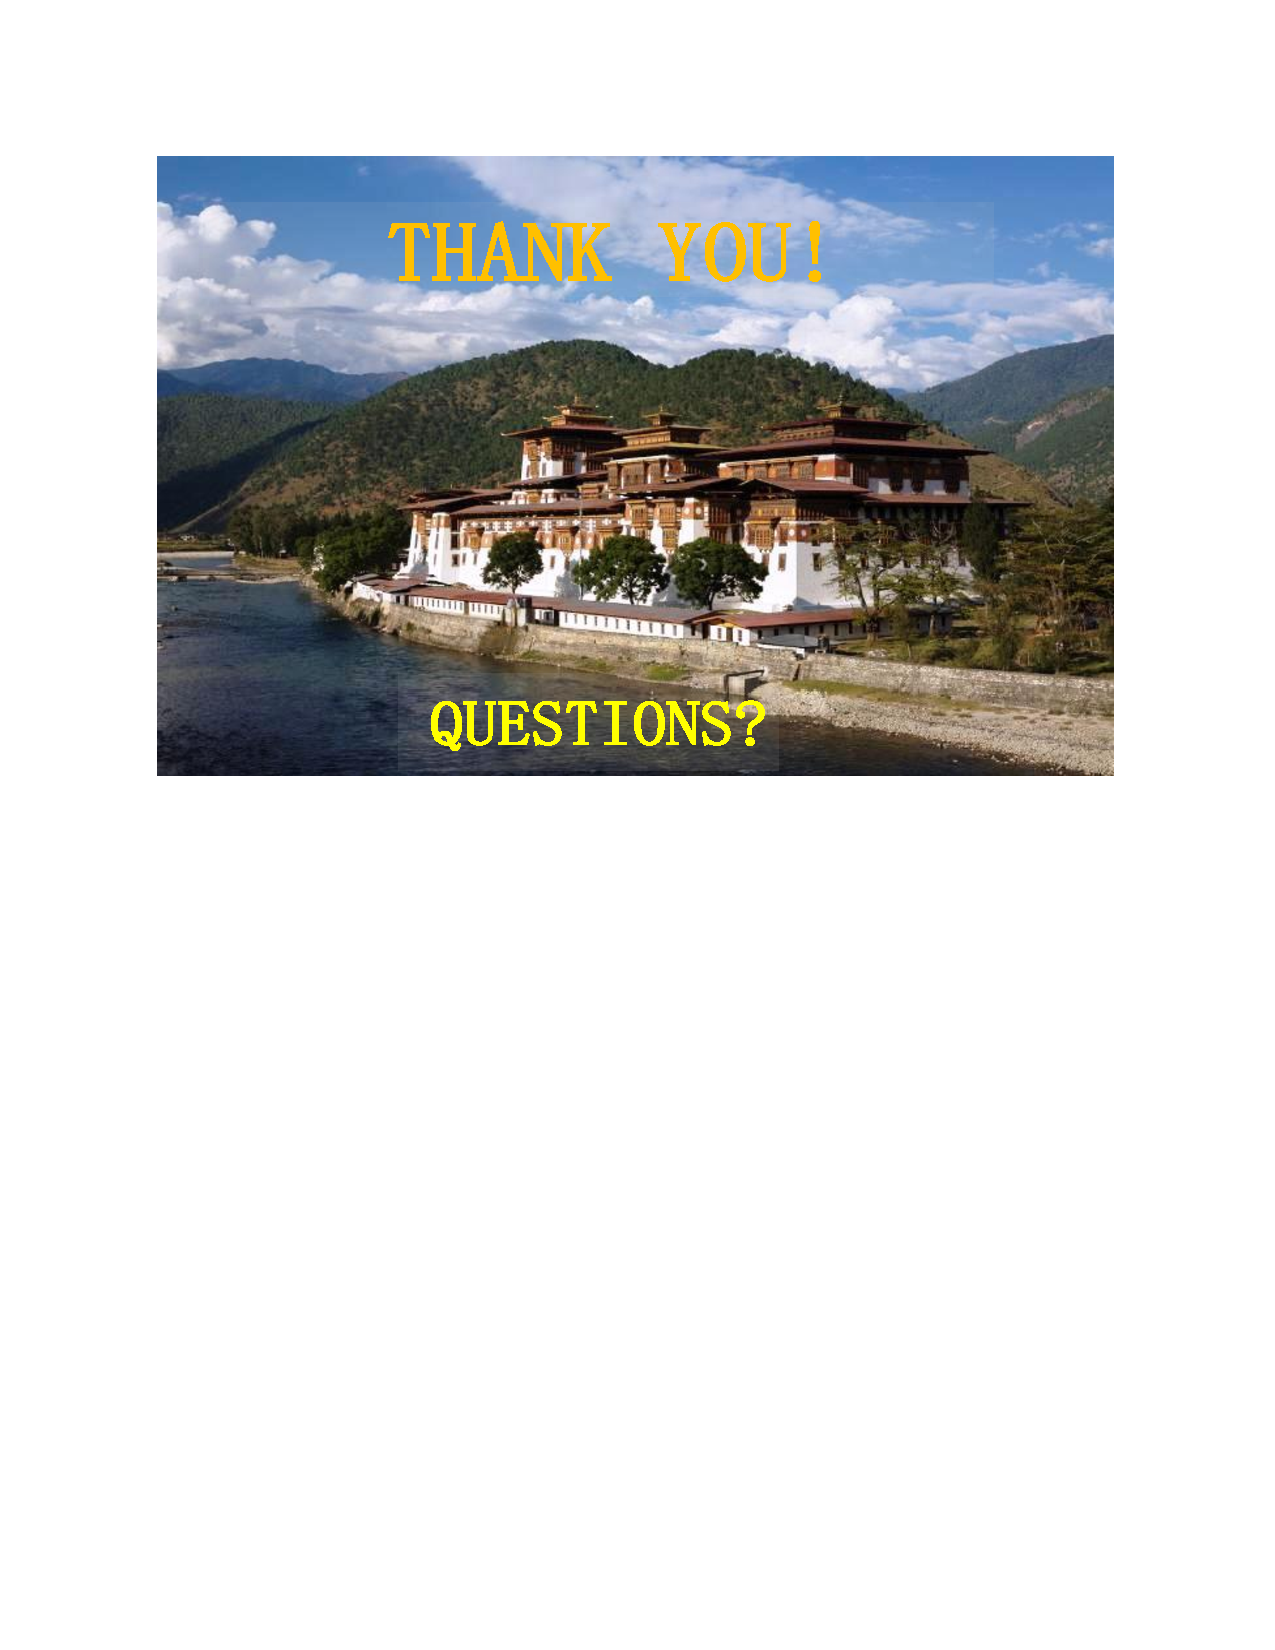
\includegraphics[width=10cm, height=6cm]{thanks.jpg}
%\begin{figure}
%\centering
%\item \vspace{0.2cm} QUESTIONS
%\end{figure}
}
%%%%%%%%%%%%%%%%%%%%%%%%%%%%%%%%%%%%%%%%%%%%%%%%%%%%%%%%%%%%%%%%%%
\end{document}
